\chapter{Calibration Model}

In this part, we first explicit gaussian template build a dot detection model that can detect dots in calibration plate. We then build a calibration model use detected dots in several image pairs and their correspond coordinate in real space. After that, we employ the model to some image pairs and compute the depth of the scenery in the images. Meanwhile, several optimizations are proposed together with the results of comparison experiments.

\section{Dot Detection Algorithm}

A common method used to calibrate a stereo vision system is to use a calibration plate. The computer vision system then needs to determine where the dots on the plate are. This can be achieved in many ways, but one of the most reliable method is the ‘Gaussian Peak’ detection method. In this approach, a 2D Gaussian object is used as a template and passed over a search region to identify peaks, in our case ‘dots’ or bright spots. 

After computing cross correlation of Gaussian template and calibration plate, all dots can be found by local maximum method, that is, a peak found in one part of the result matrix each time and set the value in this area to 0, until no more peak can be detected. Figure \ref{fig:gaussian_dis} shows the two dimensions gaussian template. We compute the cross correlation of the template with our calibration plate and finally detect the dots with `+' mark as shown in Figure \ref{fig:dot_detect}.

\begin{figure}[h!]
	\centering
	\begin{subfigure}[t]{0.45\linewidth}
		\centering
		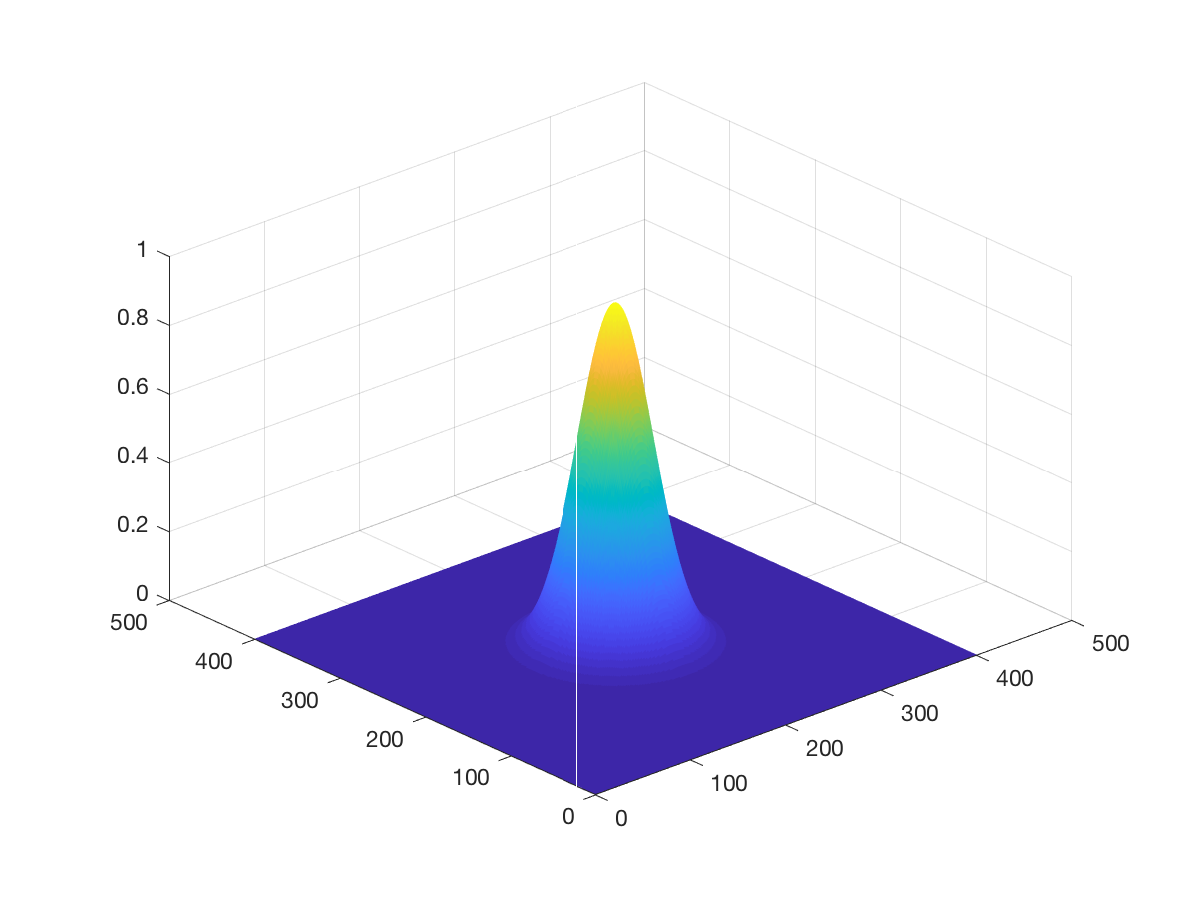
\includegraphics[width=1\linewidth]{figures/part2/gaussian_dis.eps}
		\caption{2D Gaussian}
		\label{fig:gaussian_dis}
	\end{subfigure}
	\begin{subfigure}[t]{0.45\linewidth}
		\centering
		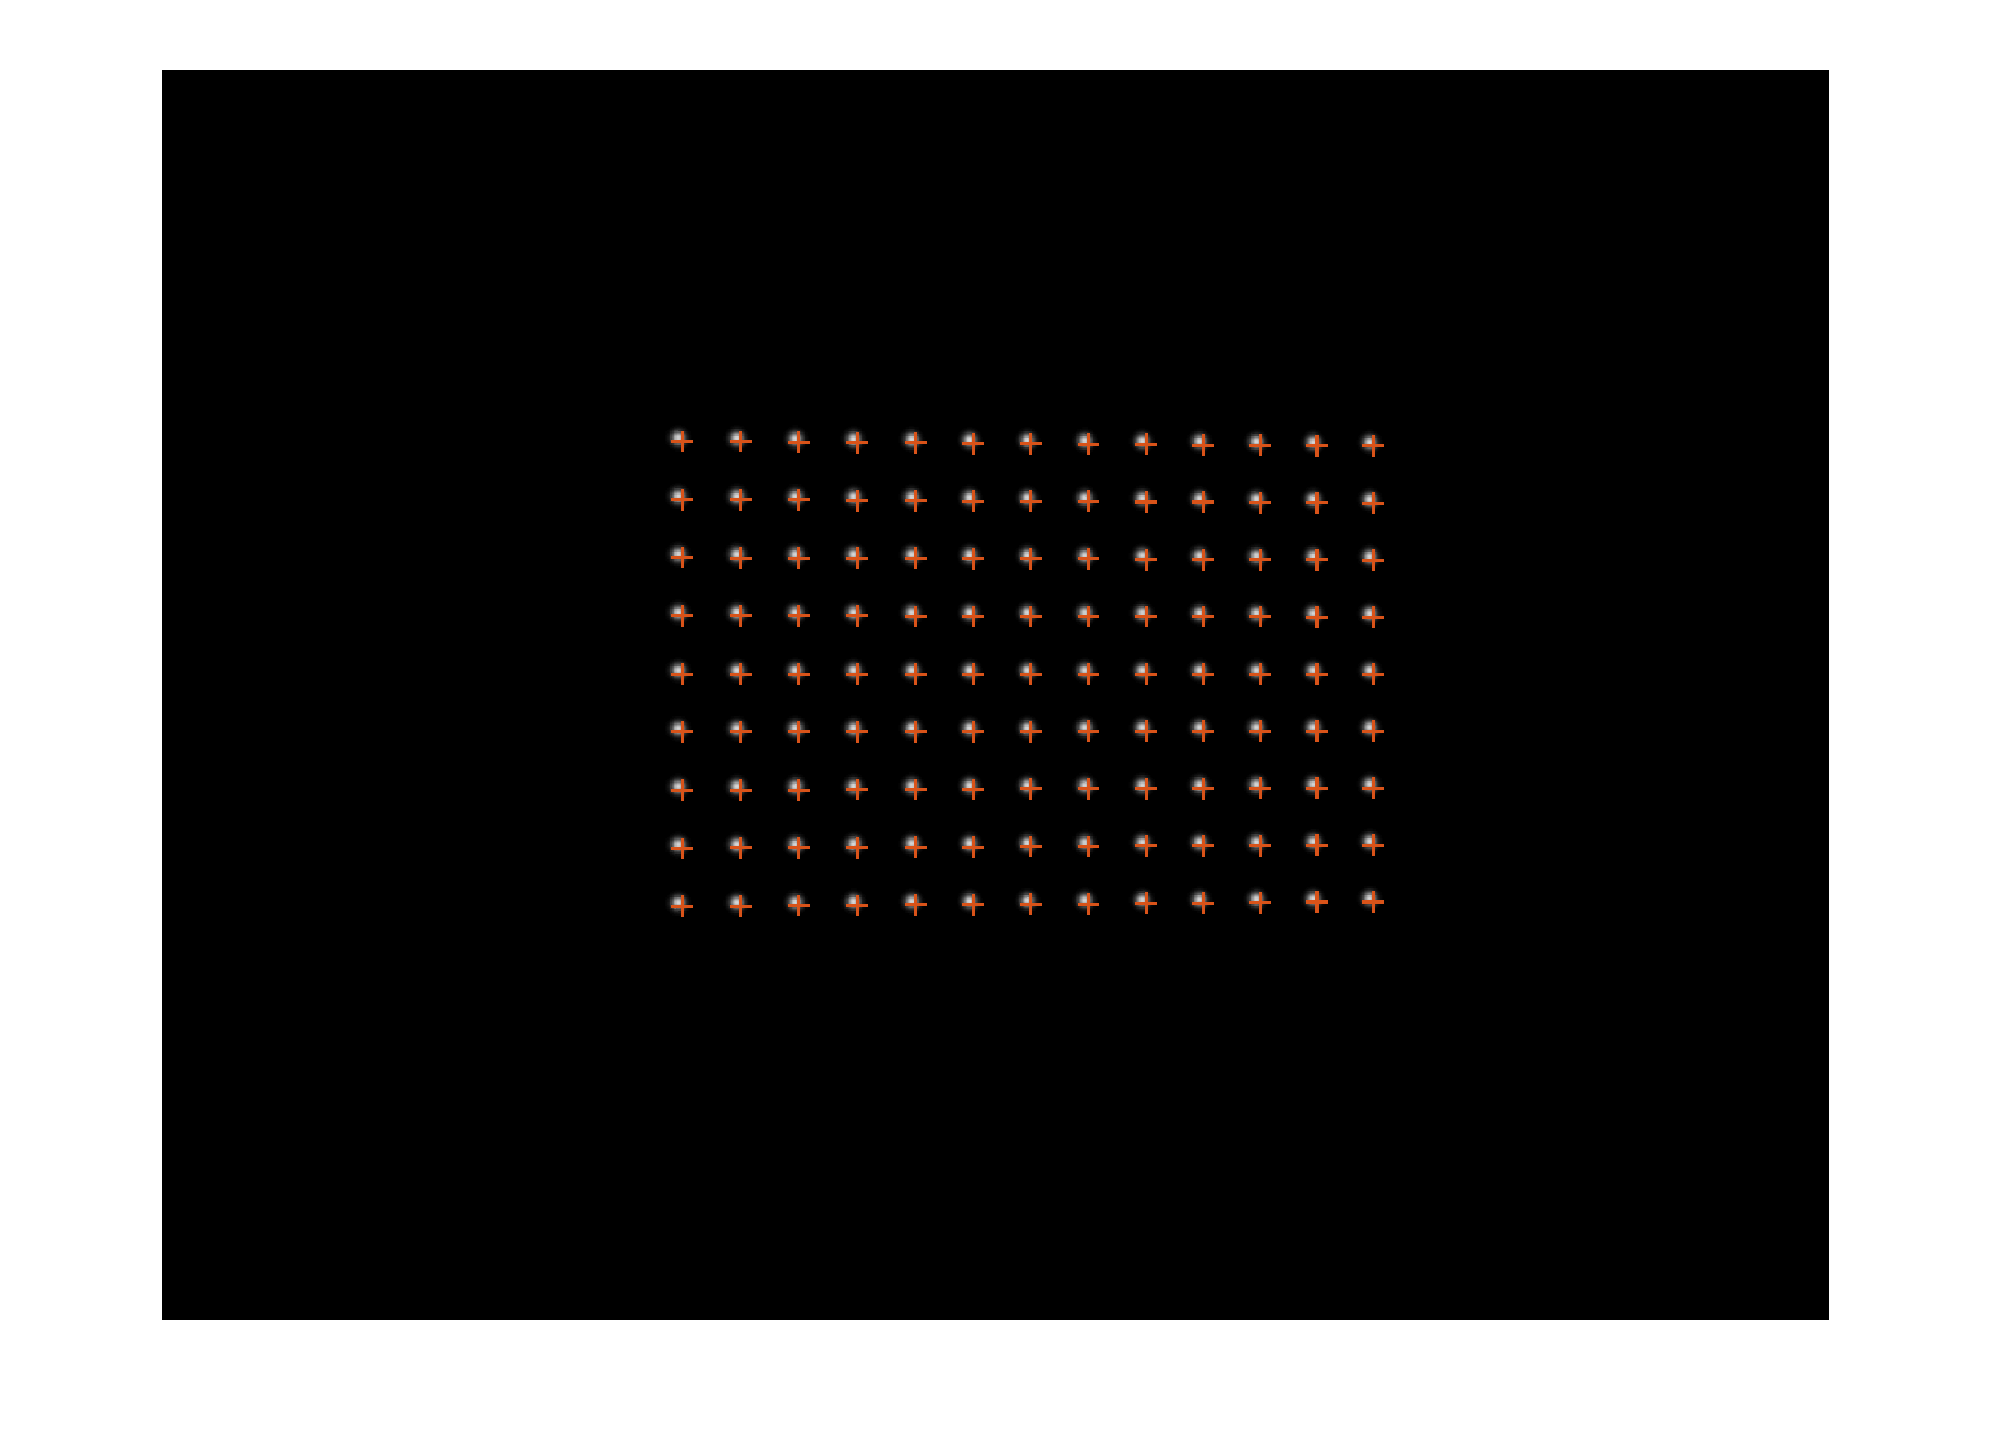
\includegraphics[width=1\linewidth]{figures/part2/dot_detect.eps}
		\caption{Dot detection results.}
		\label{fig:dot_detect}
	\end{subfigure}
	\caption{Dot detection. The original dots are bright spots in the figure (b), detected dots are marked with red cross}
\end{figure}

The detected dots are saved in the order of its been detected, as shown in Figure \ref{fig:dot_disorder}, the red line reveals the order of the dots detected. However, we need a list of dots sorted from top to bottom, left to right. Sorted dots shows in Figure \ref{fig:dot_ordered}.

\begin{figure}[h!]
	\centering
	\begin{subfigure}[t]{0.48\linewidth}
		\centering
		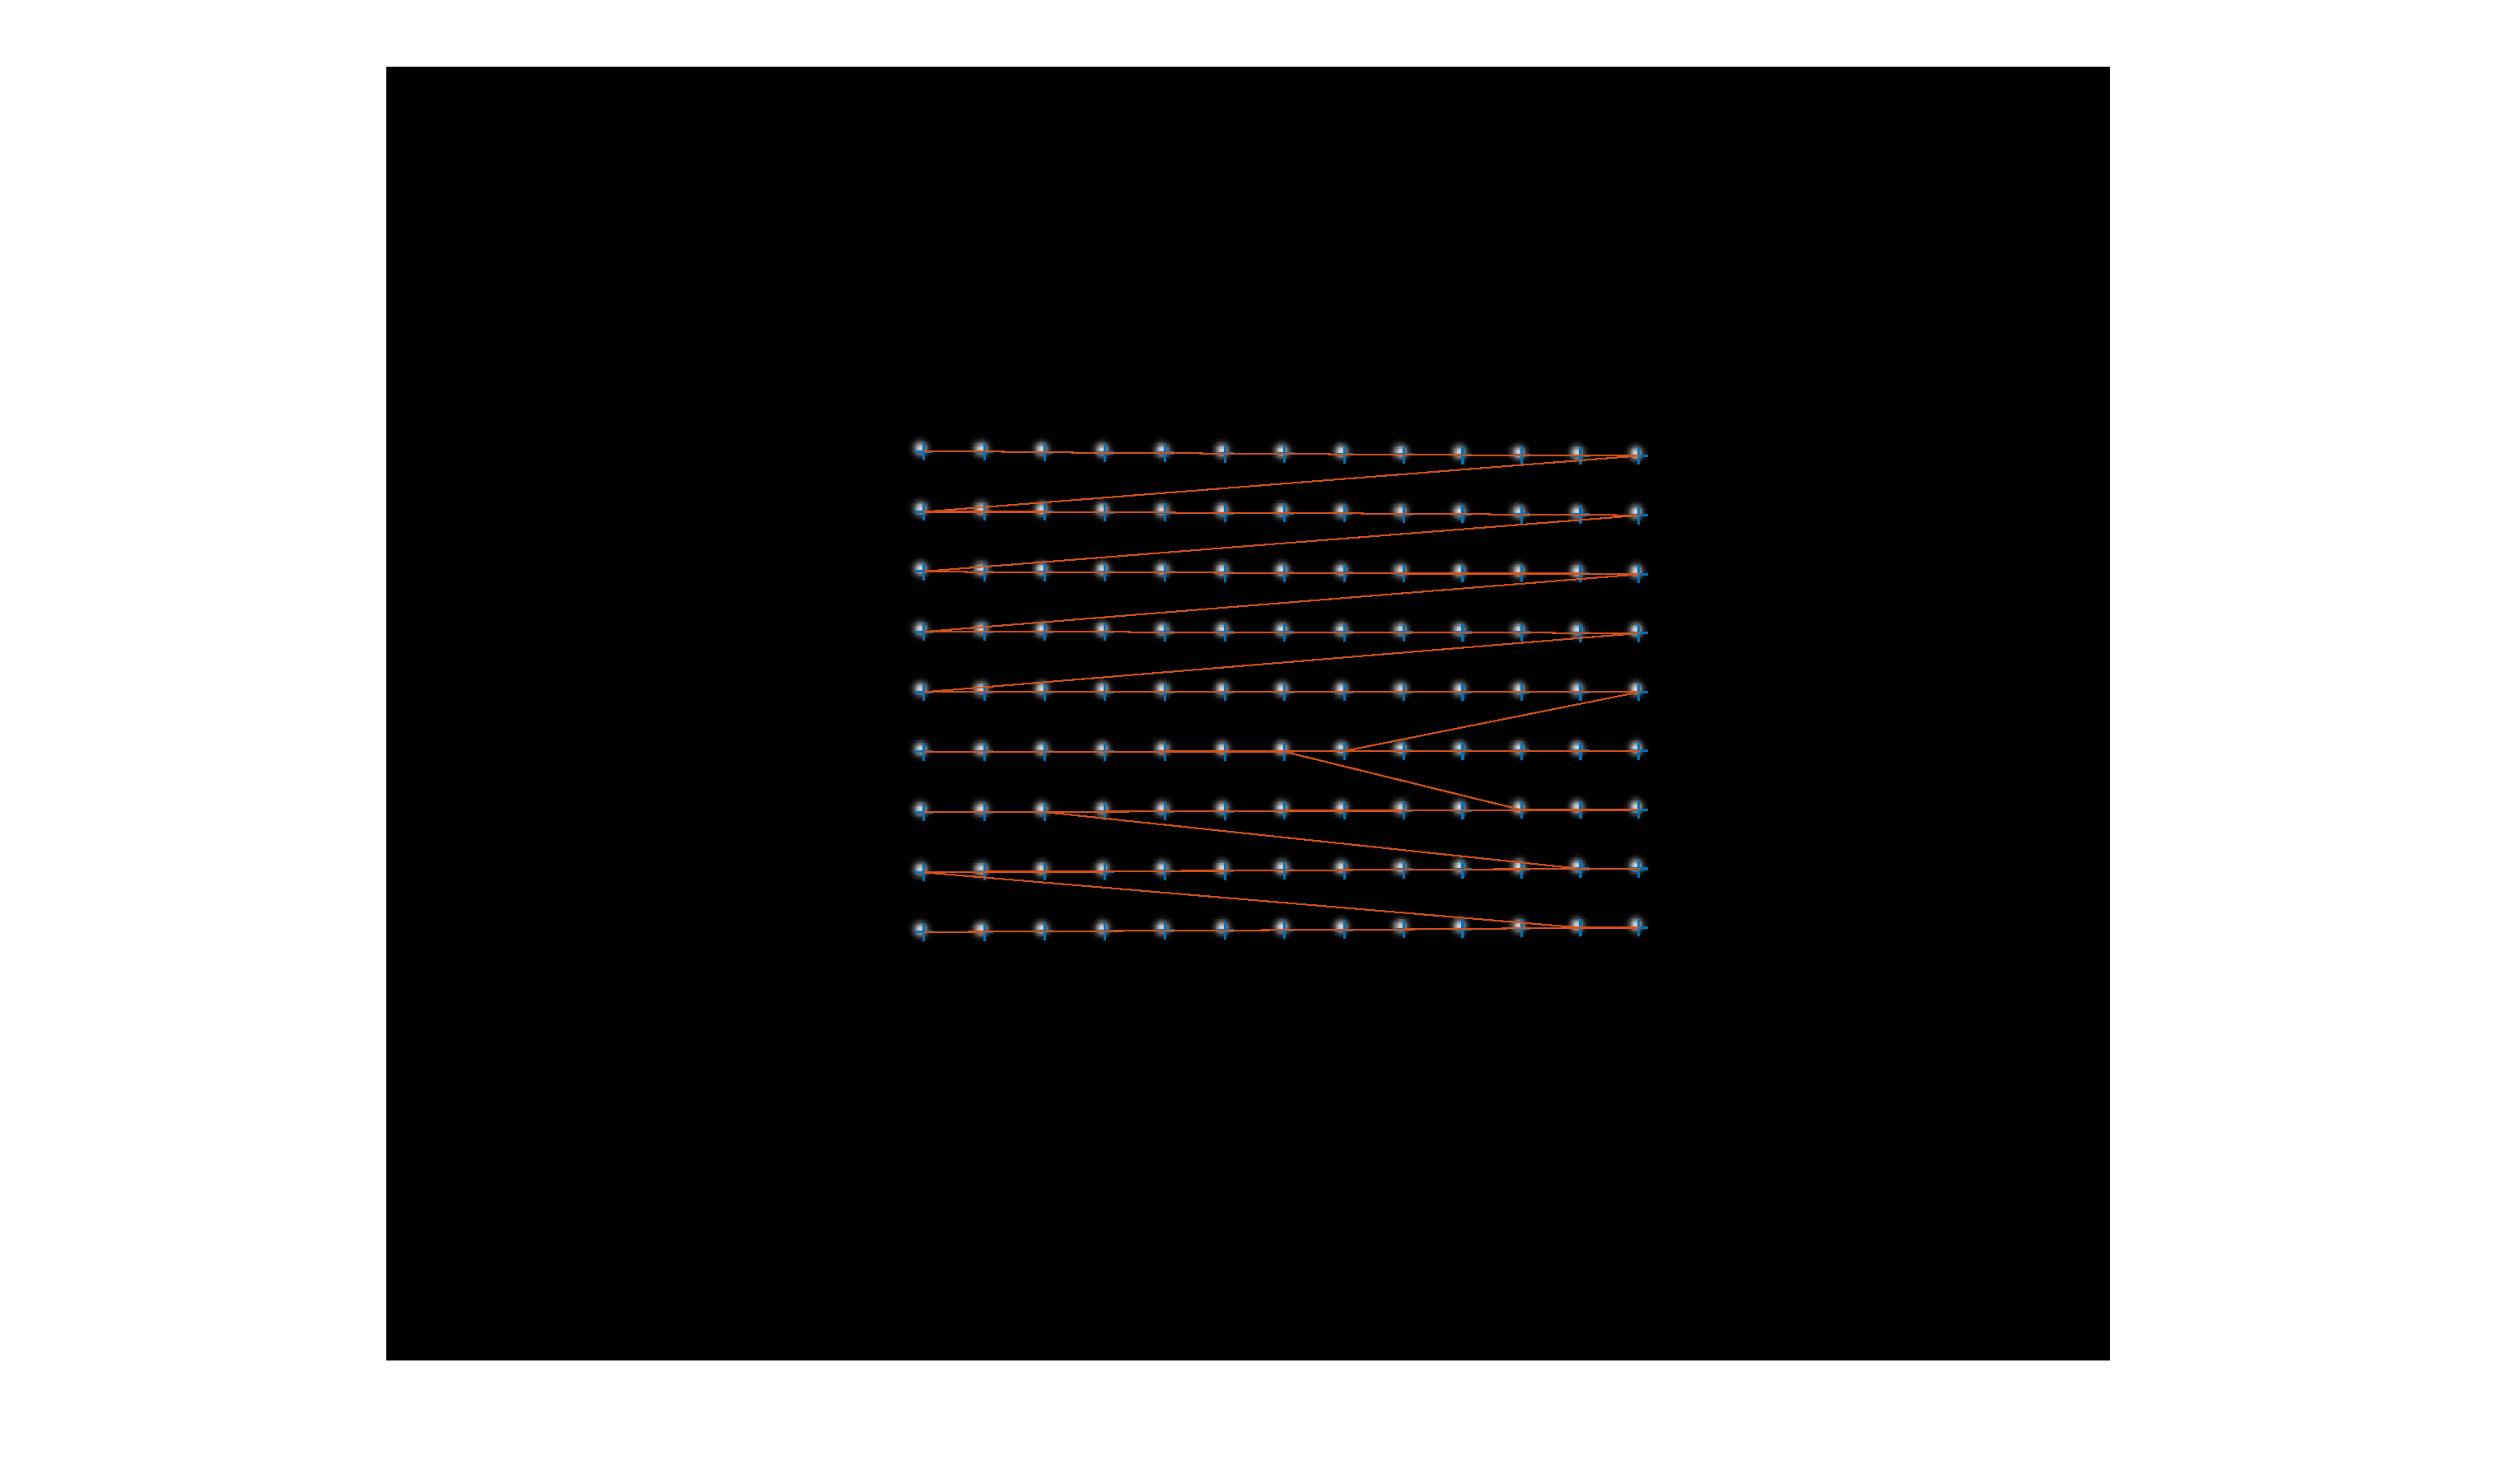
\includegraphics[width=1\linewidth]{figures/part2/dot_disorder.eps}
		\caption{Disordered dots}
		\label{fig:dot_disorder}
	\end{subfigure}
	\begin{subfigure}[t]{0.48\linewidth}
		\centering
		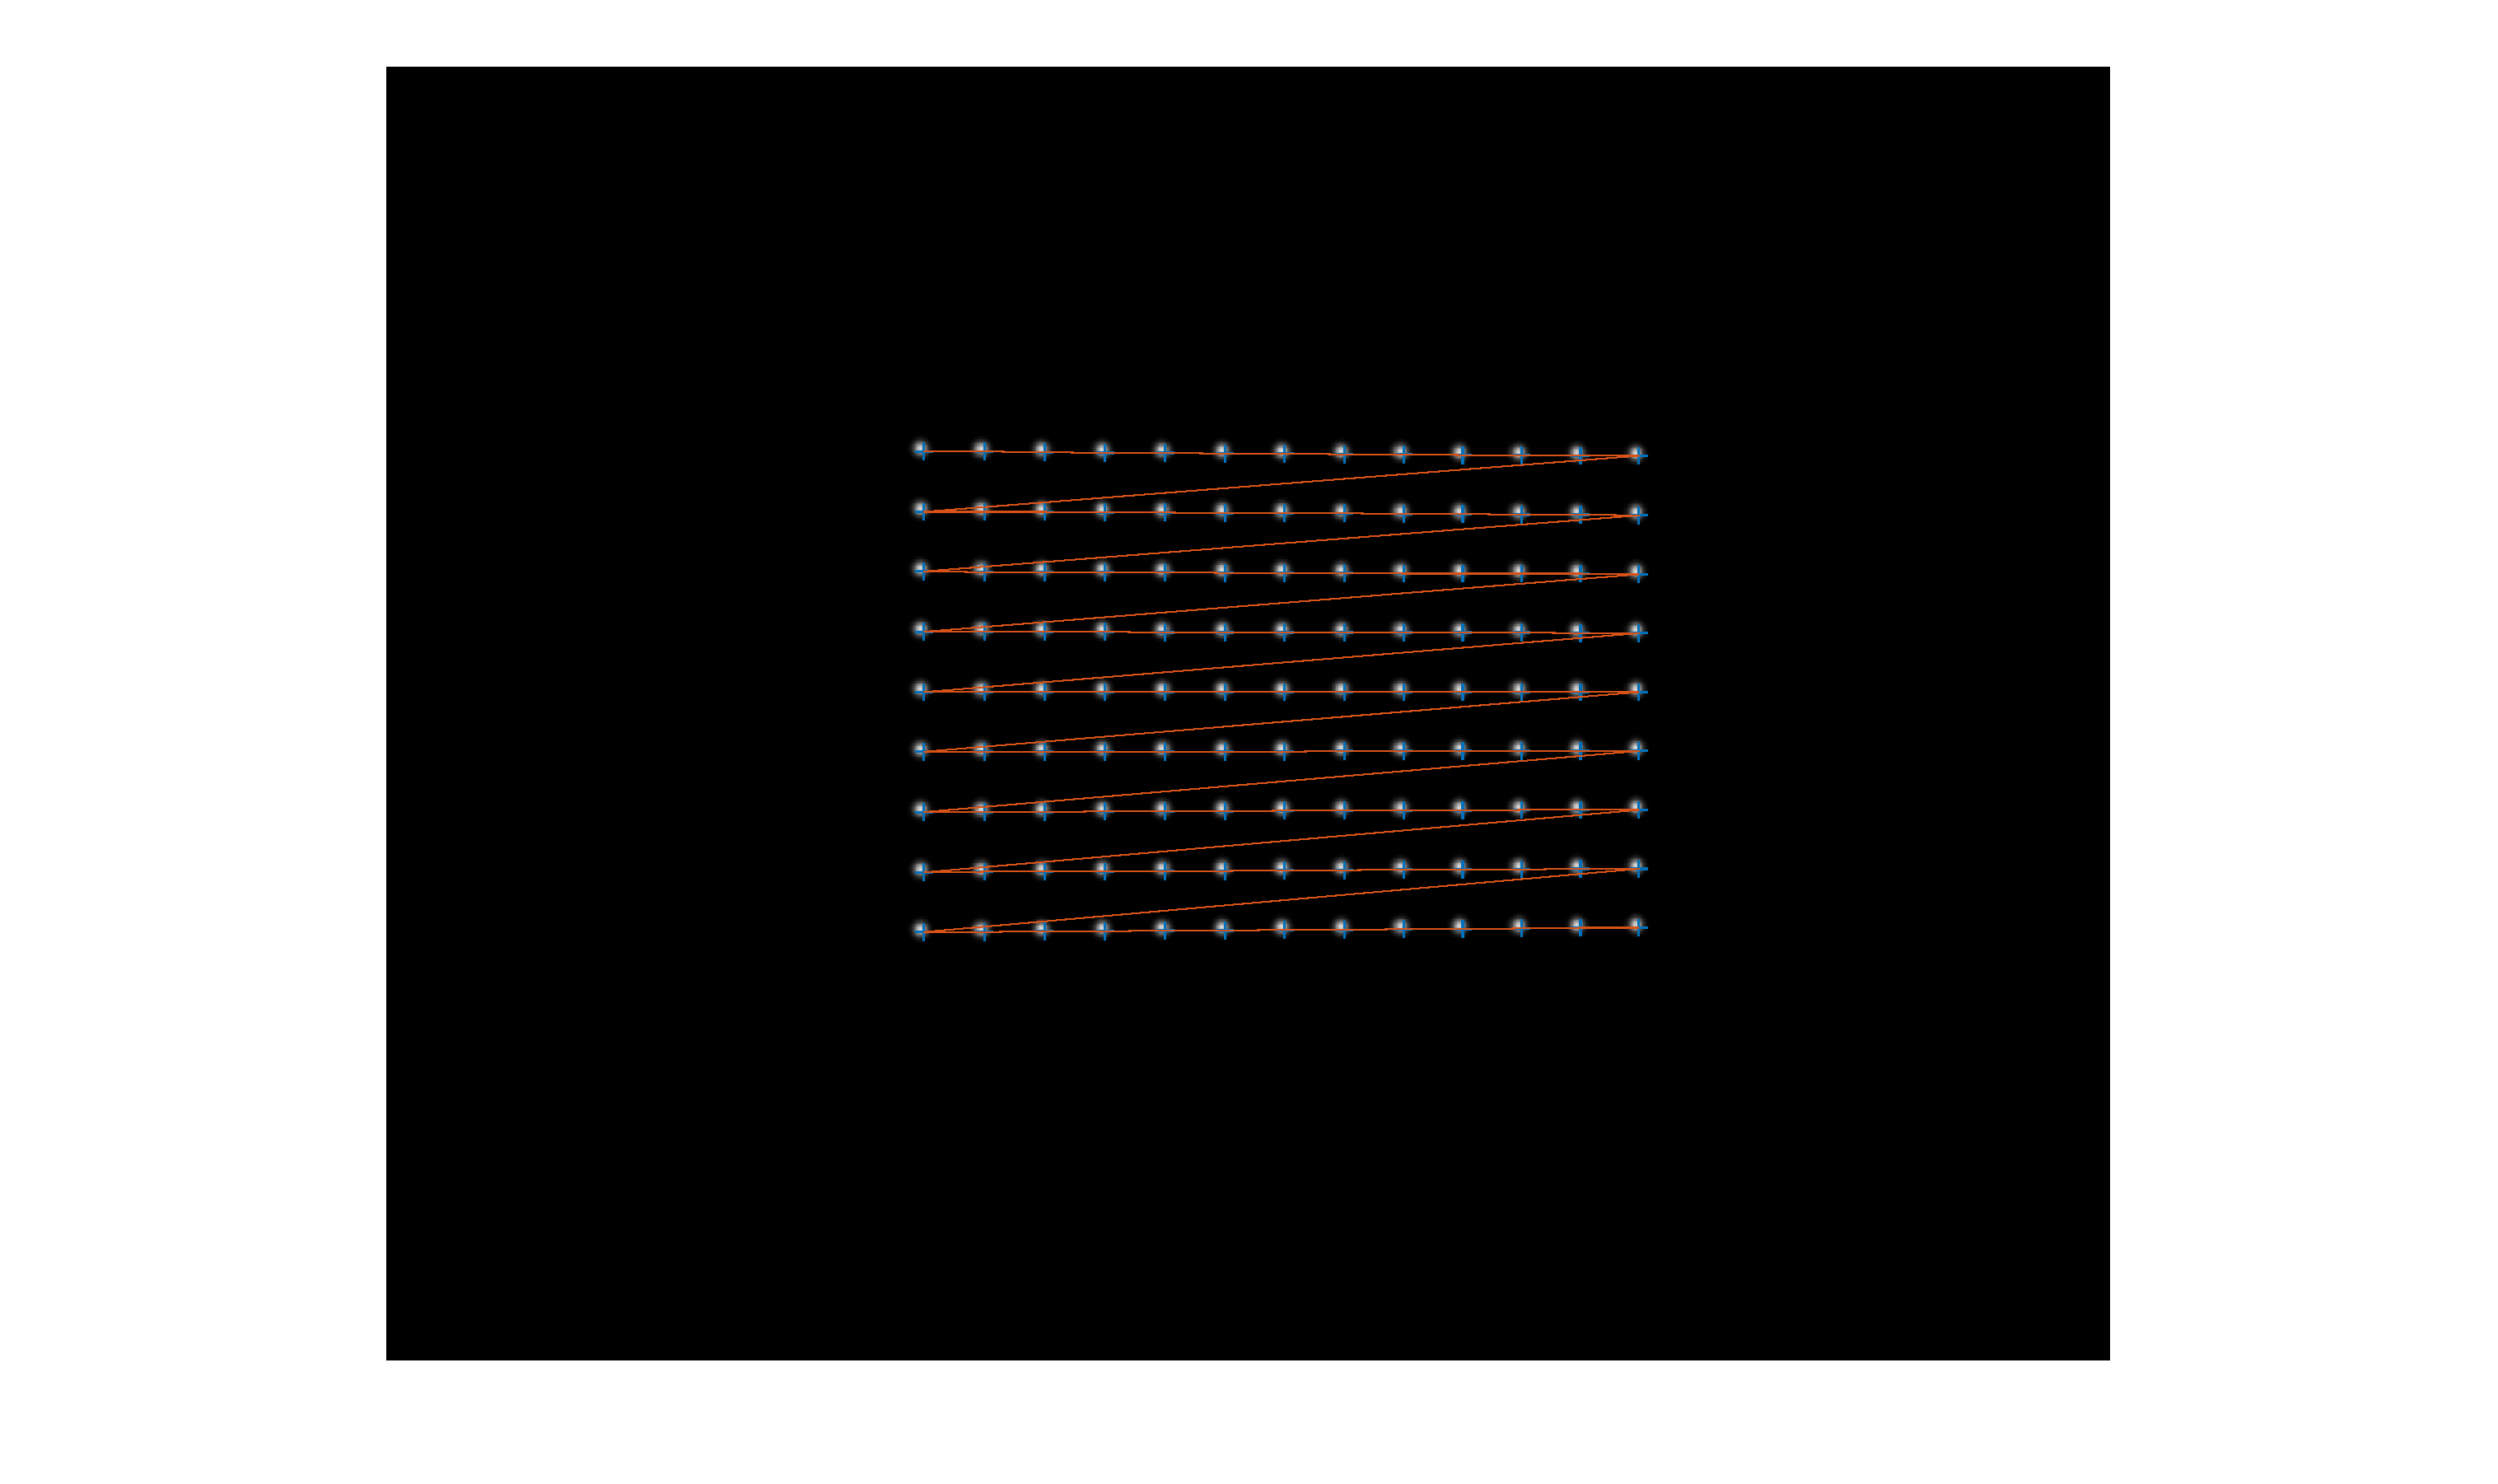
\includegraphics[width=1\linewidth]{figures/part2/dot_ordered.eps}
		\caption{Ordered dots}
		\label{fig:dot_ordered}
	\end{subfigure}
	\caption{Sort dots from top to bottom, left to right.}
\end{figure}

Source code of Gaussian template matching, dot detection algorithm and dot sort are in Appendix \ref{code:2.1}.

\section{Create Calibration Model}

The next step is to create a program which imports all the calibration images and records the pixel and real locations of all dots in each image. We use a fitting tool to create a 4D surface fit which connects all pixel space to real space within the calibrated zone. In this task, we have several calibration samples. Each sample contains two images, they are from a left and right camera, viewing the same calibration target at a stereo angle of approximately $\pm9^{\circ}$. The calibration target has white dots spaced by 50 mm in the x (horizontal) and y (vertical) directions and it is shifted to various z locations with the given distance that away from the cameras. Therefore the location of the dots in real place will be known as well as the location in the left and right images can also be detected in task 1. Figure \ref{fig:extrinsic} demonstrates the mechanism of calibration model. In this figure, $O$ and $O'$ are two cameras and $X$ is the object.

\begin{figure}[h!]
	\centering
	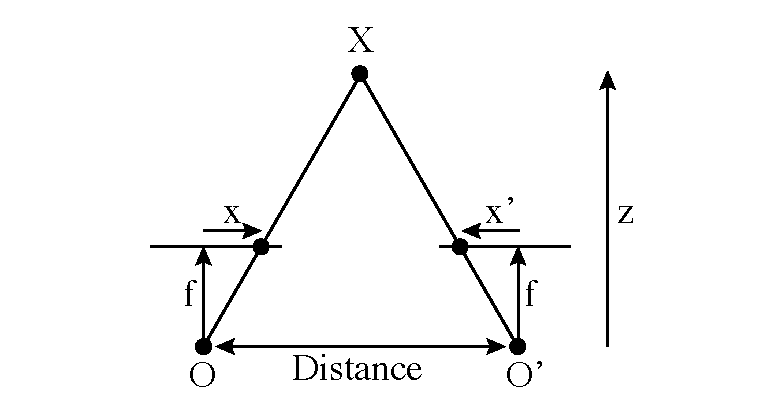
\includegraphics[width=0.6\linewidth]{figures/part2/extrinsic}
	\caption{Calibration model mechanism and extrinsic parameters calculation.}
	\label{fig:extrinsic}
\end{figure}

We use Matlab method \texttt{polyfitn} to build three fit functions for $x,y$ and $z$ coordinates in real space by using corresponding calibrate target's coordinates in left and right images, as

\begin{equation*}
	\centering
	x_{real} = f_{1}(x_{left}, y_{left}, x_{right}, y_{right}) 
\end{equation*}
\begin{equation*}
	\centering
	y_{real} = f_{2}(x_{left}, y_{left}, x_{right}, y_{right}) 
\end{equation*}
\begin{equation*}
	\centering
	z_{real} = f_{3}(x_{left}, y_{left}, x_{right}, y_{right}) 
\end{equation*}

Besides, we can get more extrinsic parameters like camera's location and orientation in the world. In Figure \ref{fig:extrinsic}, the distance between cameras and object $z$ and the distance between image planes and a lens (which provides a transformation between object space and image space) $f$ are known, $x$ and $x'$ are available from two taken pictures. So we can calculate the distance between two cameras through triangle similarity theorems.

Source code of calibration model creation is in Appendix \ref{code:2.2}.

\section{Image Comparison}

After build calibration model. We hope to test the performance of our model using a pair of general images. But the images taken by cameras are not dots with certain distribution rules. Preprocess of the image is needed before applying it to our calibration model. 

As observed in Chapter \ref{chp:1}, the cross correlation technique can sensitively and accurately identify patterns in complex images. Consider the two views of Physics South Building in Melbourne University, as shown in Figure \ref{fig:mel}. As humans, most of us can easily recognize that both images are of the same scene, just taken from different angles or positions. But our computers can not thinking like human so that image comparison must be done for matching objects in the two views. 

\begin{figure}[h!]
	\centering
	\begin{subfigure}[t]{0.48\linewidth}
		\centering
		\includegraphics[width=1\linewidth]{figures/part2/mel_left}
		\caption{Left view}
		\label{fig:mel_left}
	\end{subfigure}
	\begin{subfigure}[t]{0.48\linewidth}
		\centering
		\includegraphics[width=1\linewidth]{figures/part2/mel_right}
		\caption{Right view}
		\label{fig:mel_right}
	\end{subfigure}
	\caption{Template created in left image (orange), search region created in right image (3 times larger than template, centered at the same pixel location).}
	\label{fig:mel}
\end{figure}

Firstly, let one image broken up in to windows and create a template from one window, like shown in Figure \ref{fig:mel_left}, then creating a search region (larger than the template) in the other image as shown in Figure \ref{fig:mel_right}. Additionally, scanning the template around the search region is able to find similar feature using cross correlation, in general as well as get the position of max correlation and compute the difference in pixel location (disparity). Repeat this for all windows and then we can get all corresponding positions which is very similar with the corresponding dots we detected in task 1.

The search region is 9 times larger than template in this task. However, for a more general task, exhaustively search the space of right view images ensure the best match to be found. But this method is time consuming. therefore, speeding up at the risk of possible failure to find the best match is used. Actually, there is better image comparison technique that makes use of spatial intensity gradient of the image\cite{Lucas1981An}, and more methods \cite{Marr1988A}, \cite{Moravec1980Obstacle}.

The result of image comparison shows in Figure \ref{fig:img_cmp}. From which we find that most divided regions have a relatively high disparity. The reason may be that the images are taken by myself so that the distance between two cameras are long and they do not keep in a same high level.

\begin{figure}[h!]
	\centering
	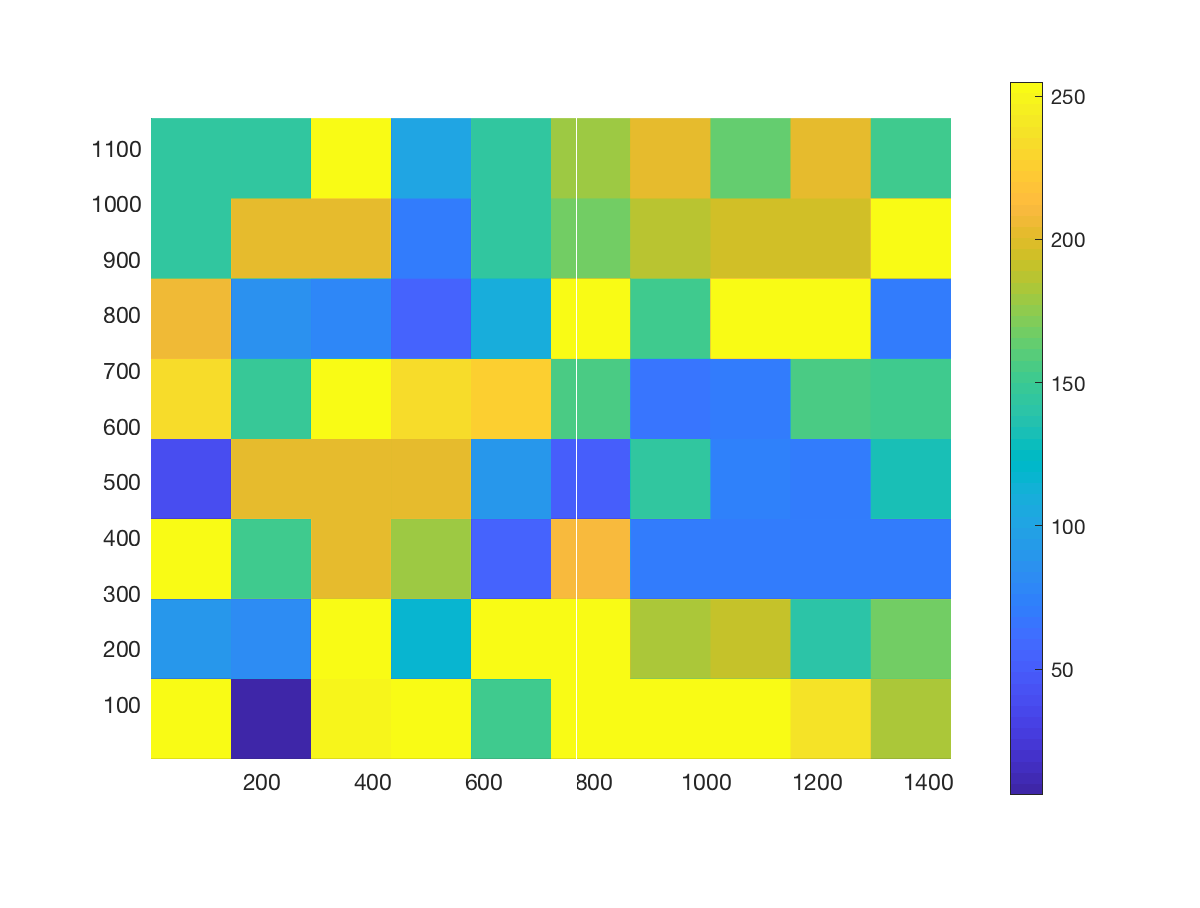
\includegraphics[width=0.5\linewidth]{figures/part2/img_cmp}
	\caption{Image compare result, the region with color higher on the colorbar means the higher disparity}
	\label{fig:img_cmp}
\end{figure}

For better demonstrate image comparison. We compare two particular images collected from a standard stereo vision image set. Figure \ref{fig:img_cmp1} shows the results. From which we can find the smaller windows size, the more information we can get. Another obvious phenomenon is the regions near to corner of the images tend to have high disparities cause these regions are pure black in left compared image so that it is hard to find a precise matched region in right image. Moreover, as the search region is set only 3 times larger than the template, smaller windows may result in more templates that can not find a good match in the right view images. This problem will be solved in next task.

\begin{figure}[h!]
	\centering
	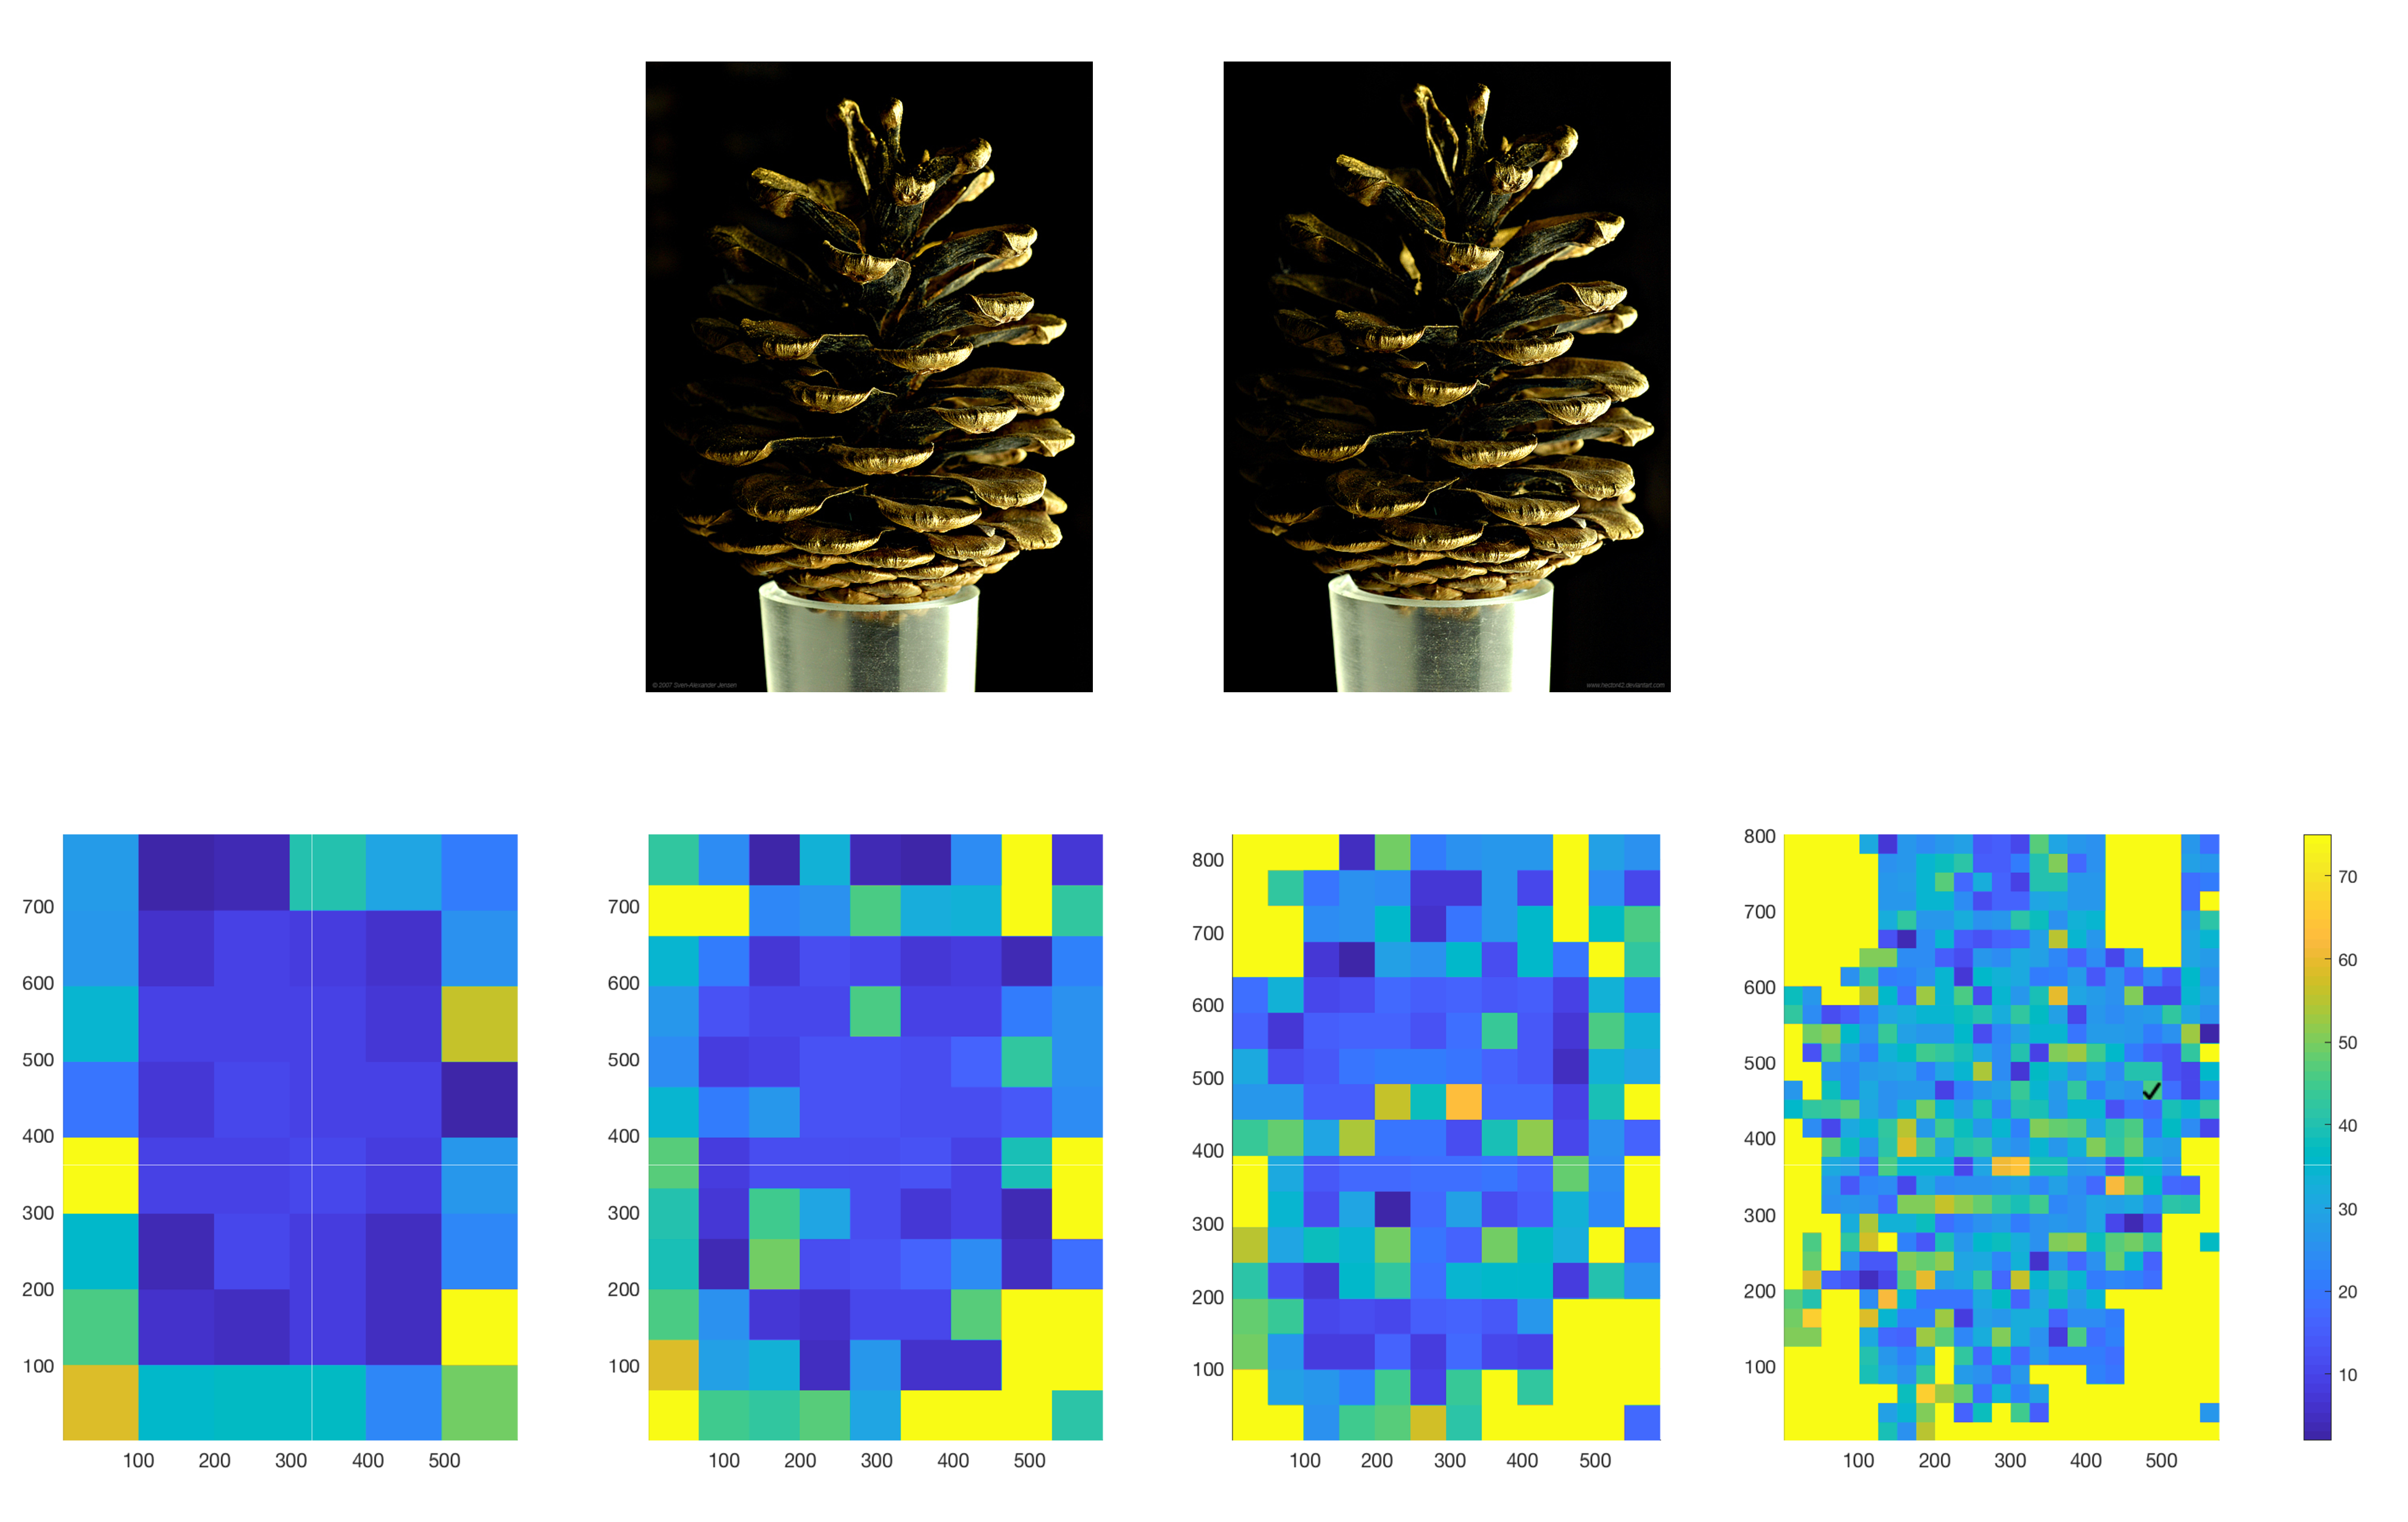
\includegraphics[width=1\linewidth]{figures/part2/img_cmp1}
	\caption{First two images are the image be compared, other four are results of different window size.}
	\label{fig:img_cmp1}
\end{figure}

Source code about image comparison and result visualization are in Appendix \ref{code:2.3}.

\section{Cross Correlation Optimization}

There are several parameters, which need to be considered when applying the cross correlation technique. These include what is the ideal sized window to be used, and how best should it be scanned in search of matching. In this part, we investigate three optimization strategies:

\textbf{a). Variable window overlap}

The first optimization is variable window overlap. As mentioned in the last section, to do image comparison, the left image will be split to several parts and each part will be searched in the corresponding but the larger part of the right image. Variable overlap is demonstrate in Figure \ref{fig:window_overlap}, the split parts could have overlap. The most important benefit is the increase in the precision of disparity in one particular region. For example, one region will be compared only once if there is no overlap and it will compared 4 times if there are 50\% overlap, like the centre square of the right bottom part in Figure \ref{fig:window_overlap}

\begin{figure}[h!]
	\centering
	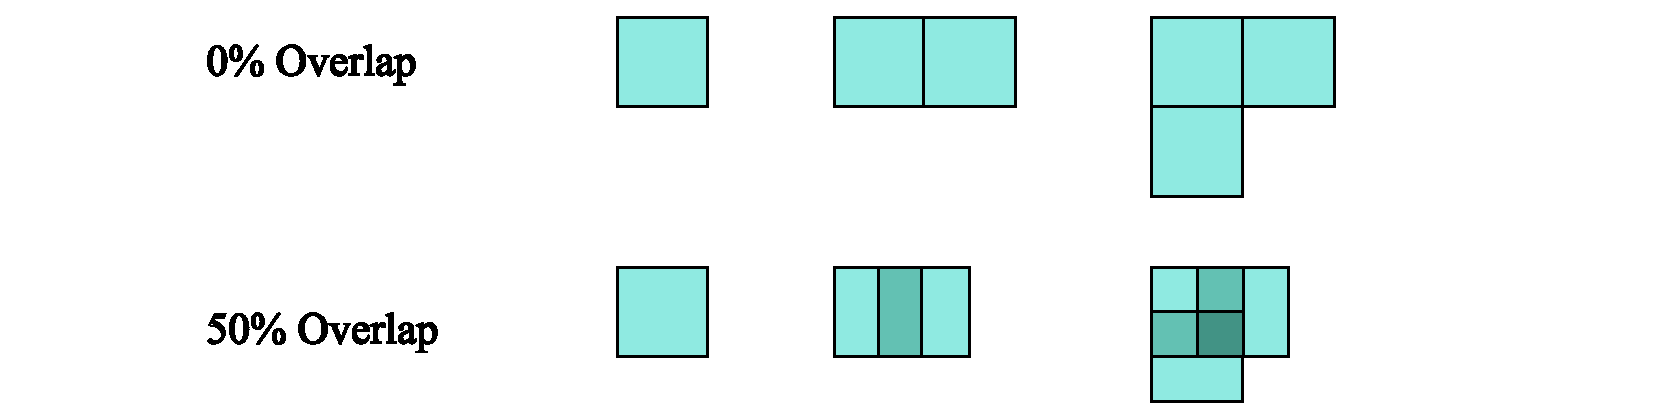
\includegraphics[width=0.8\linewidth]{figures/part2/window_overlap}
	\caption{Example of variable window overlap}
	\label{fig:window_overlap}
\end{figure}

\textbf{b).Variable search region geometry}

Variable search region geometry, shown in Figure \ref{fig:search_region}, is essential for a practical image compare model. On the one hand, if the search region is too small, the pattern may completely out of it and we can not get any useful different information. However, if search region is too big, for example, treating the complete right view image as search region, it is fairly time consuming. So a proper size of search region is essential. On the other hand, a good shape of search region is also helpful, if our images are taken in the same horizontal level, we can use flat search region rather than square region. Of course, the search region should extend in horizontal rather than vertical like shown in Figure \ref{fig:search_region}, smaller search region could save time for us.

\begin{figure}[h!]
	\centering
	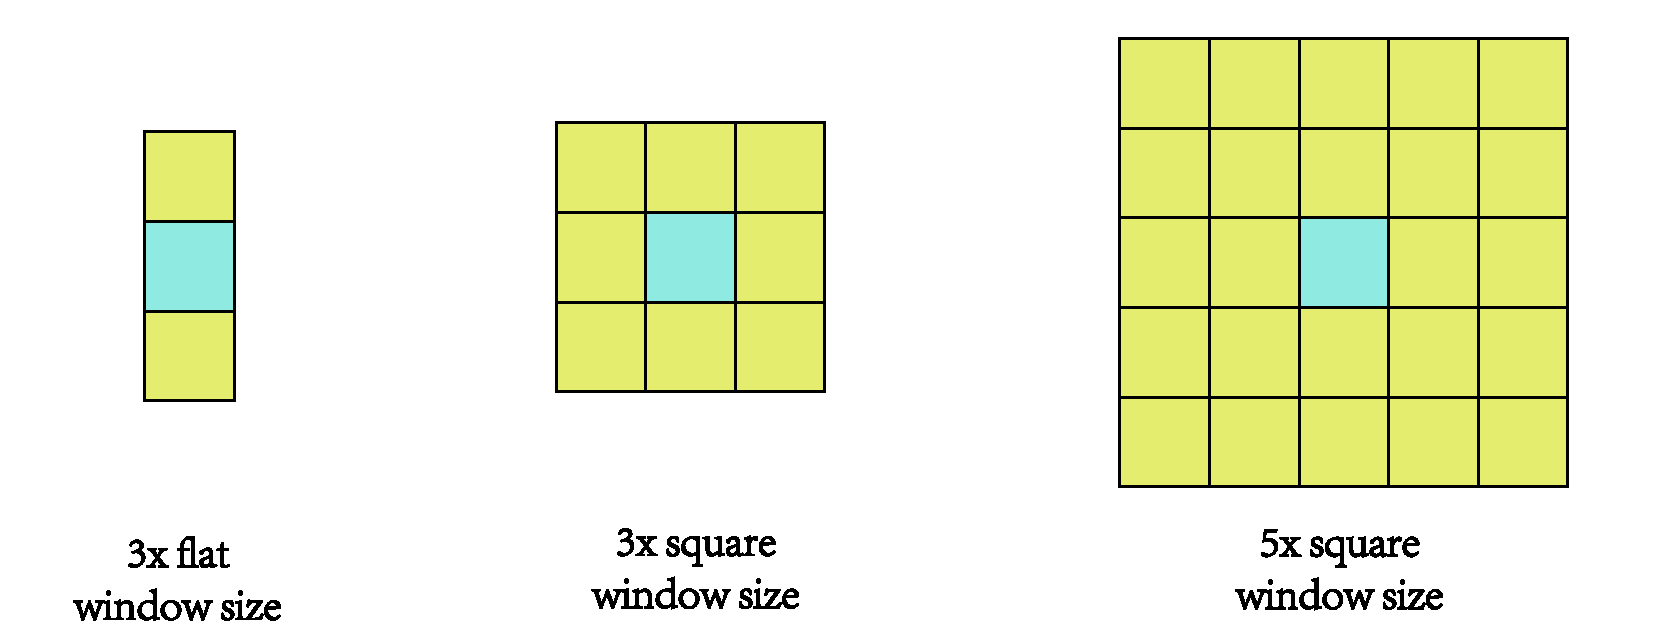
\includegraphics[width=0.8\linewidth]{figures/part2/search_region}
	\caption{Example of variable search region}
	\label{fig:search_region}
\end{figure}

Actually, what image comparison do is that for each search region in the first image, find corresponding epipolar line in the right image, and examine all pixels on the epipolar line and pick the best match. In this project, stereo cameras are parallel to each other and camera centers are at same height. Therefore, epipolar lines are fall along the horizontal scan lines of the images. Figure \ref{fig:search_region1b} shows the scan line and more reasonable search region.

\begin{figure}[h!]
	\centering
	\begin{subfigure}[t]{0.48\linewidth}
		\centering
		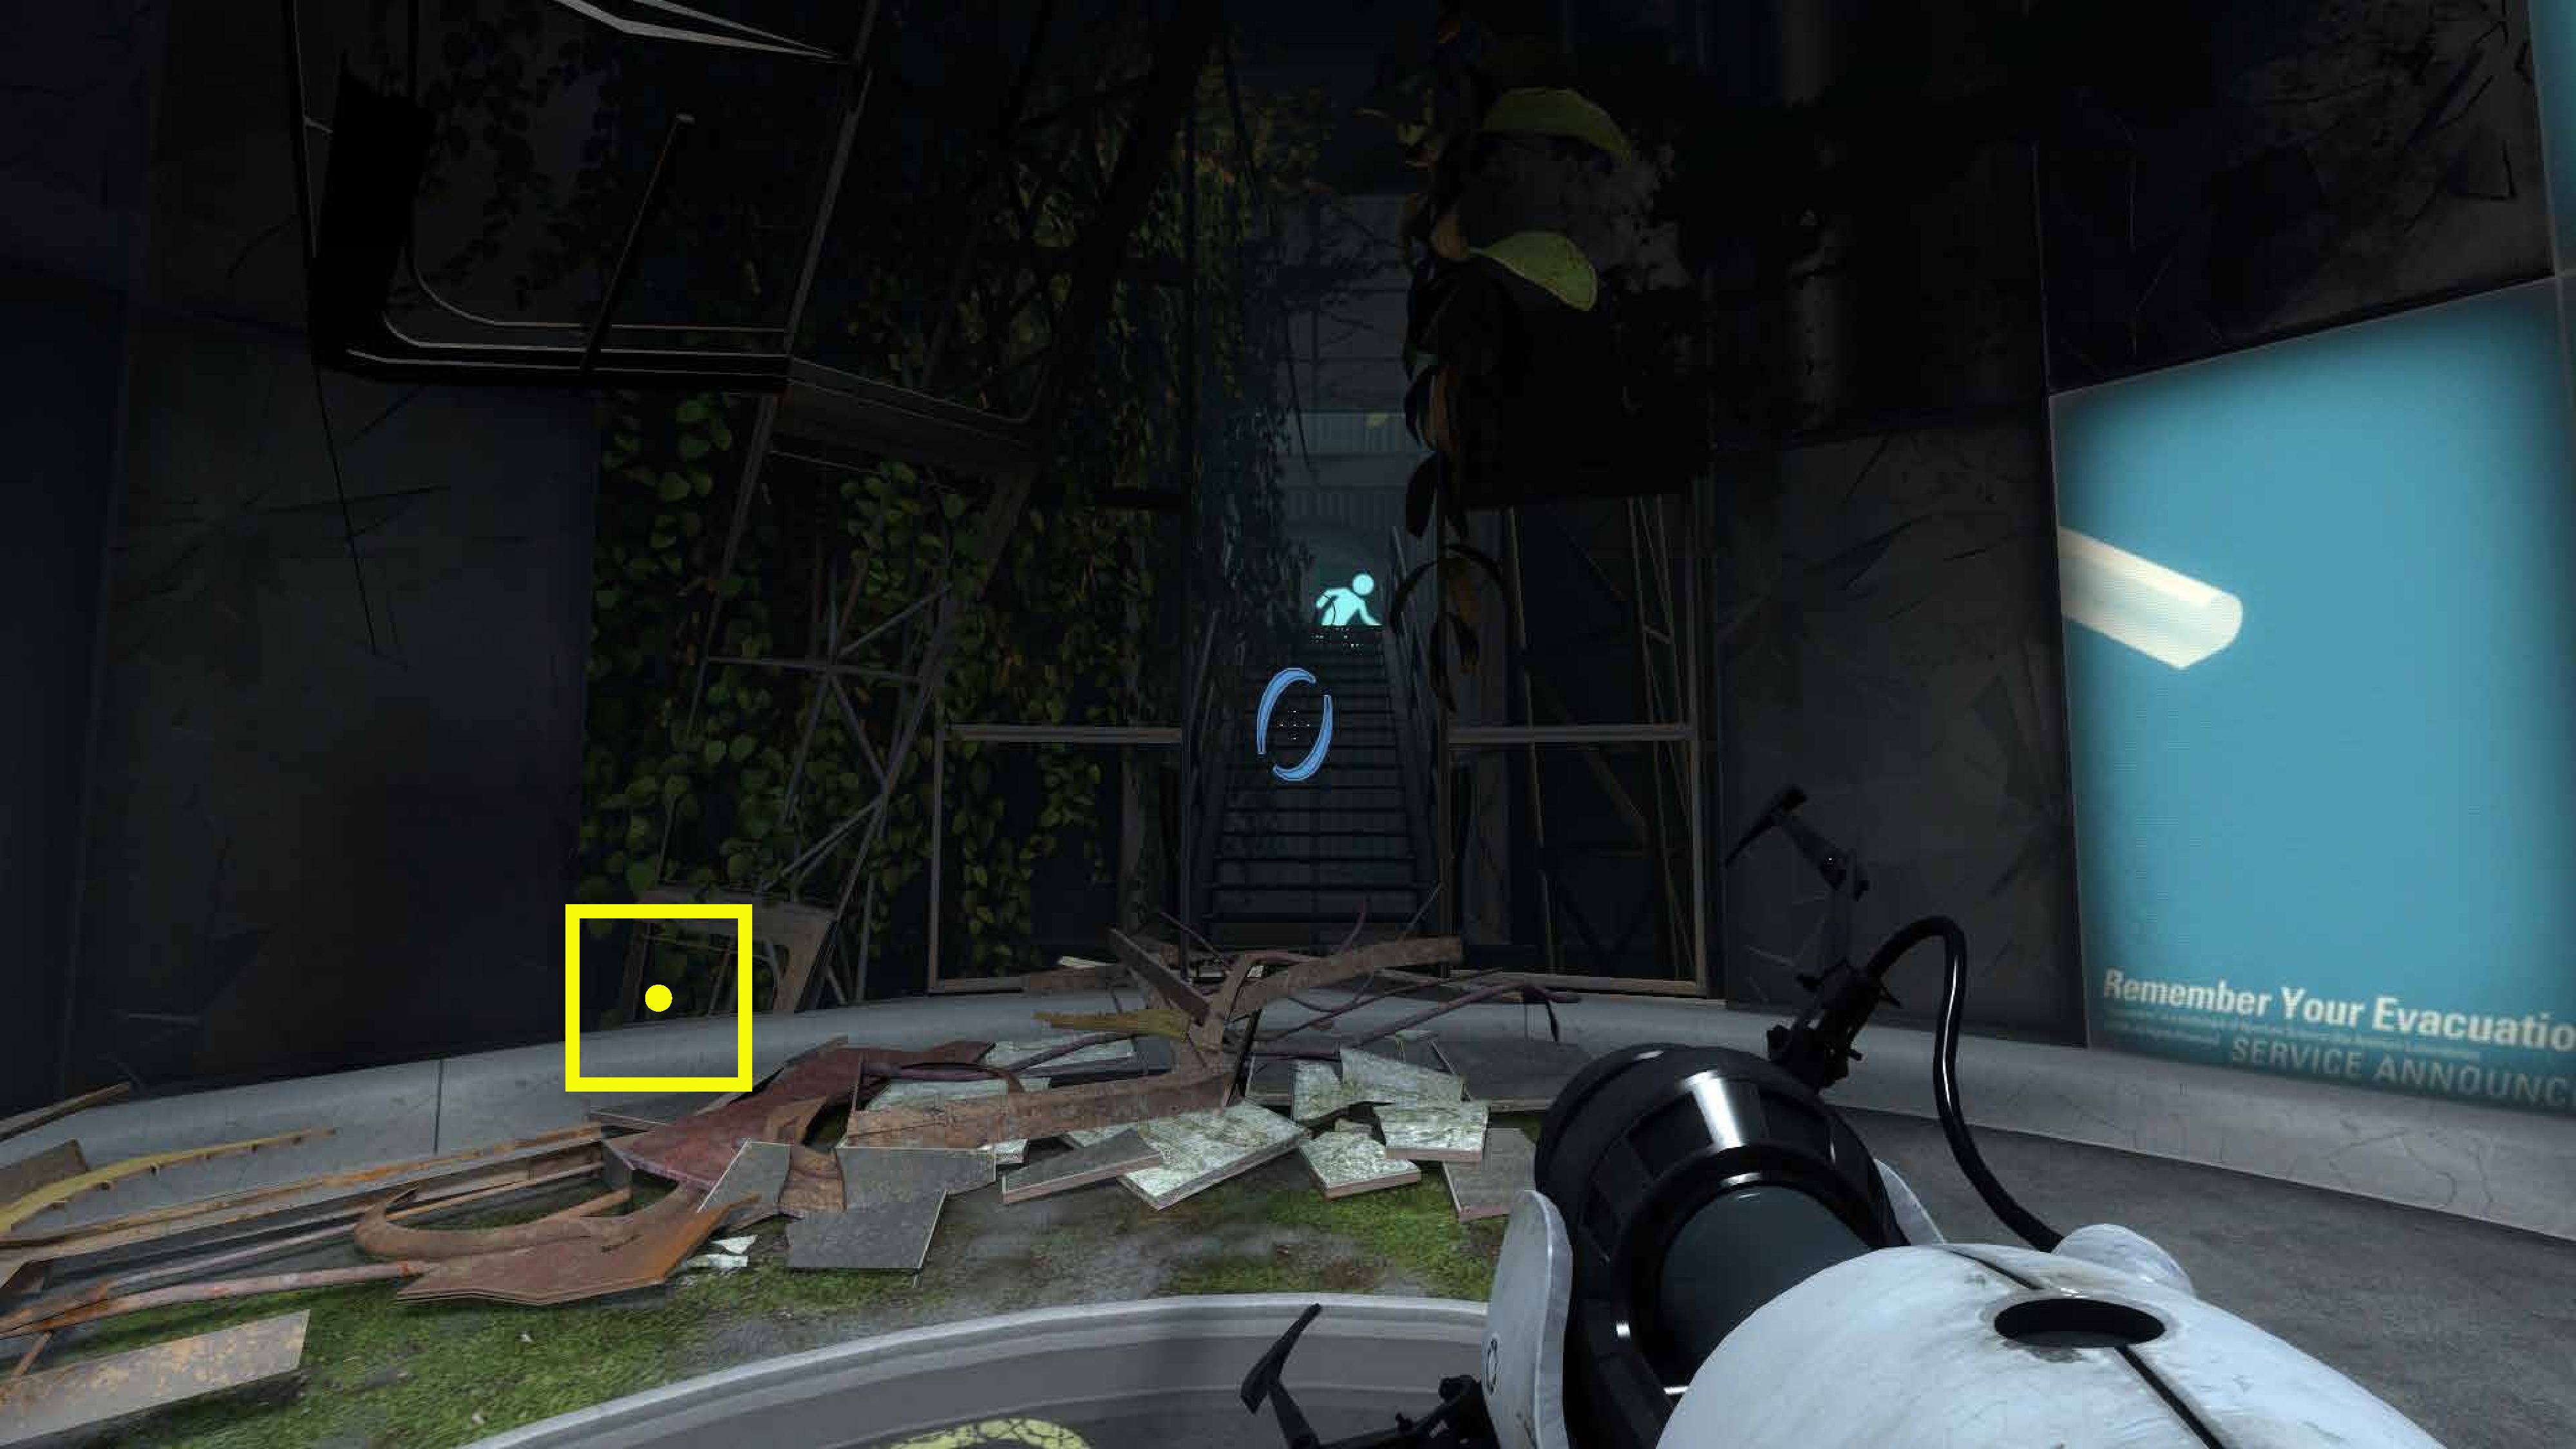
\includegraphics[width=1\linewidth]{figures/part2/search_region1a}
		\caption{Left view}
	\end{subfigure}
	\begin{subfigure}[t]{0.48\linewidth}
		\centering
		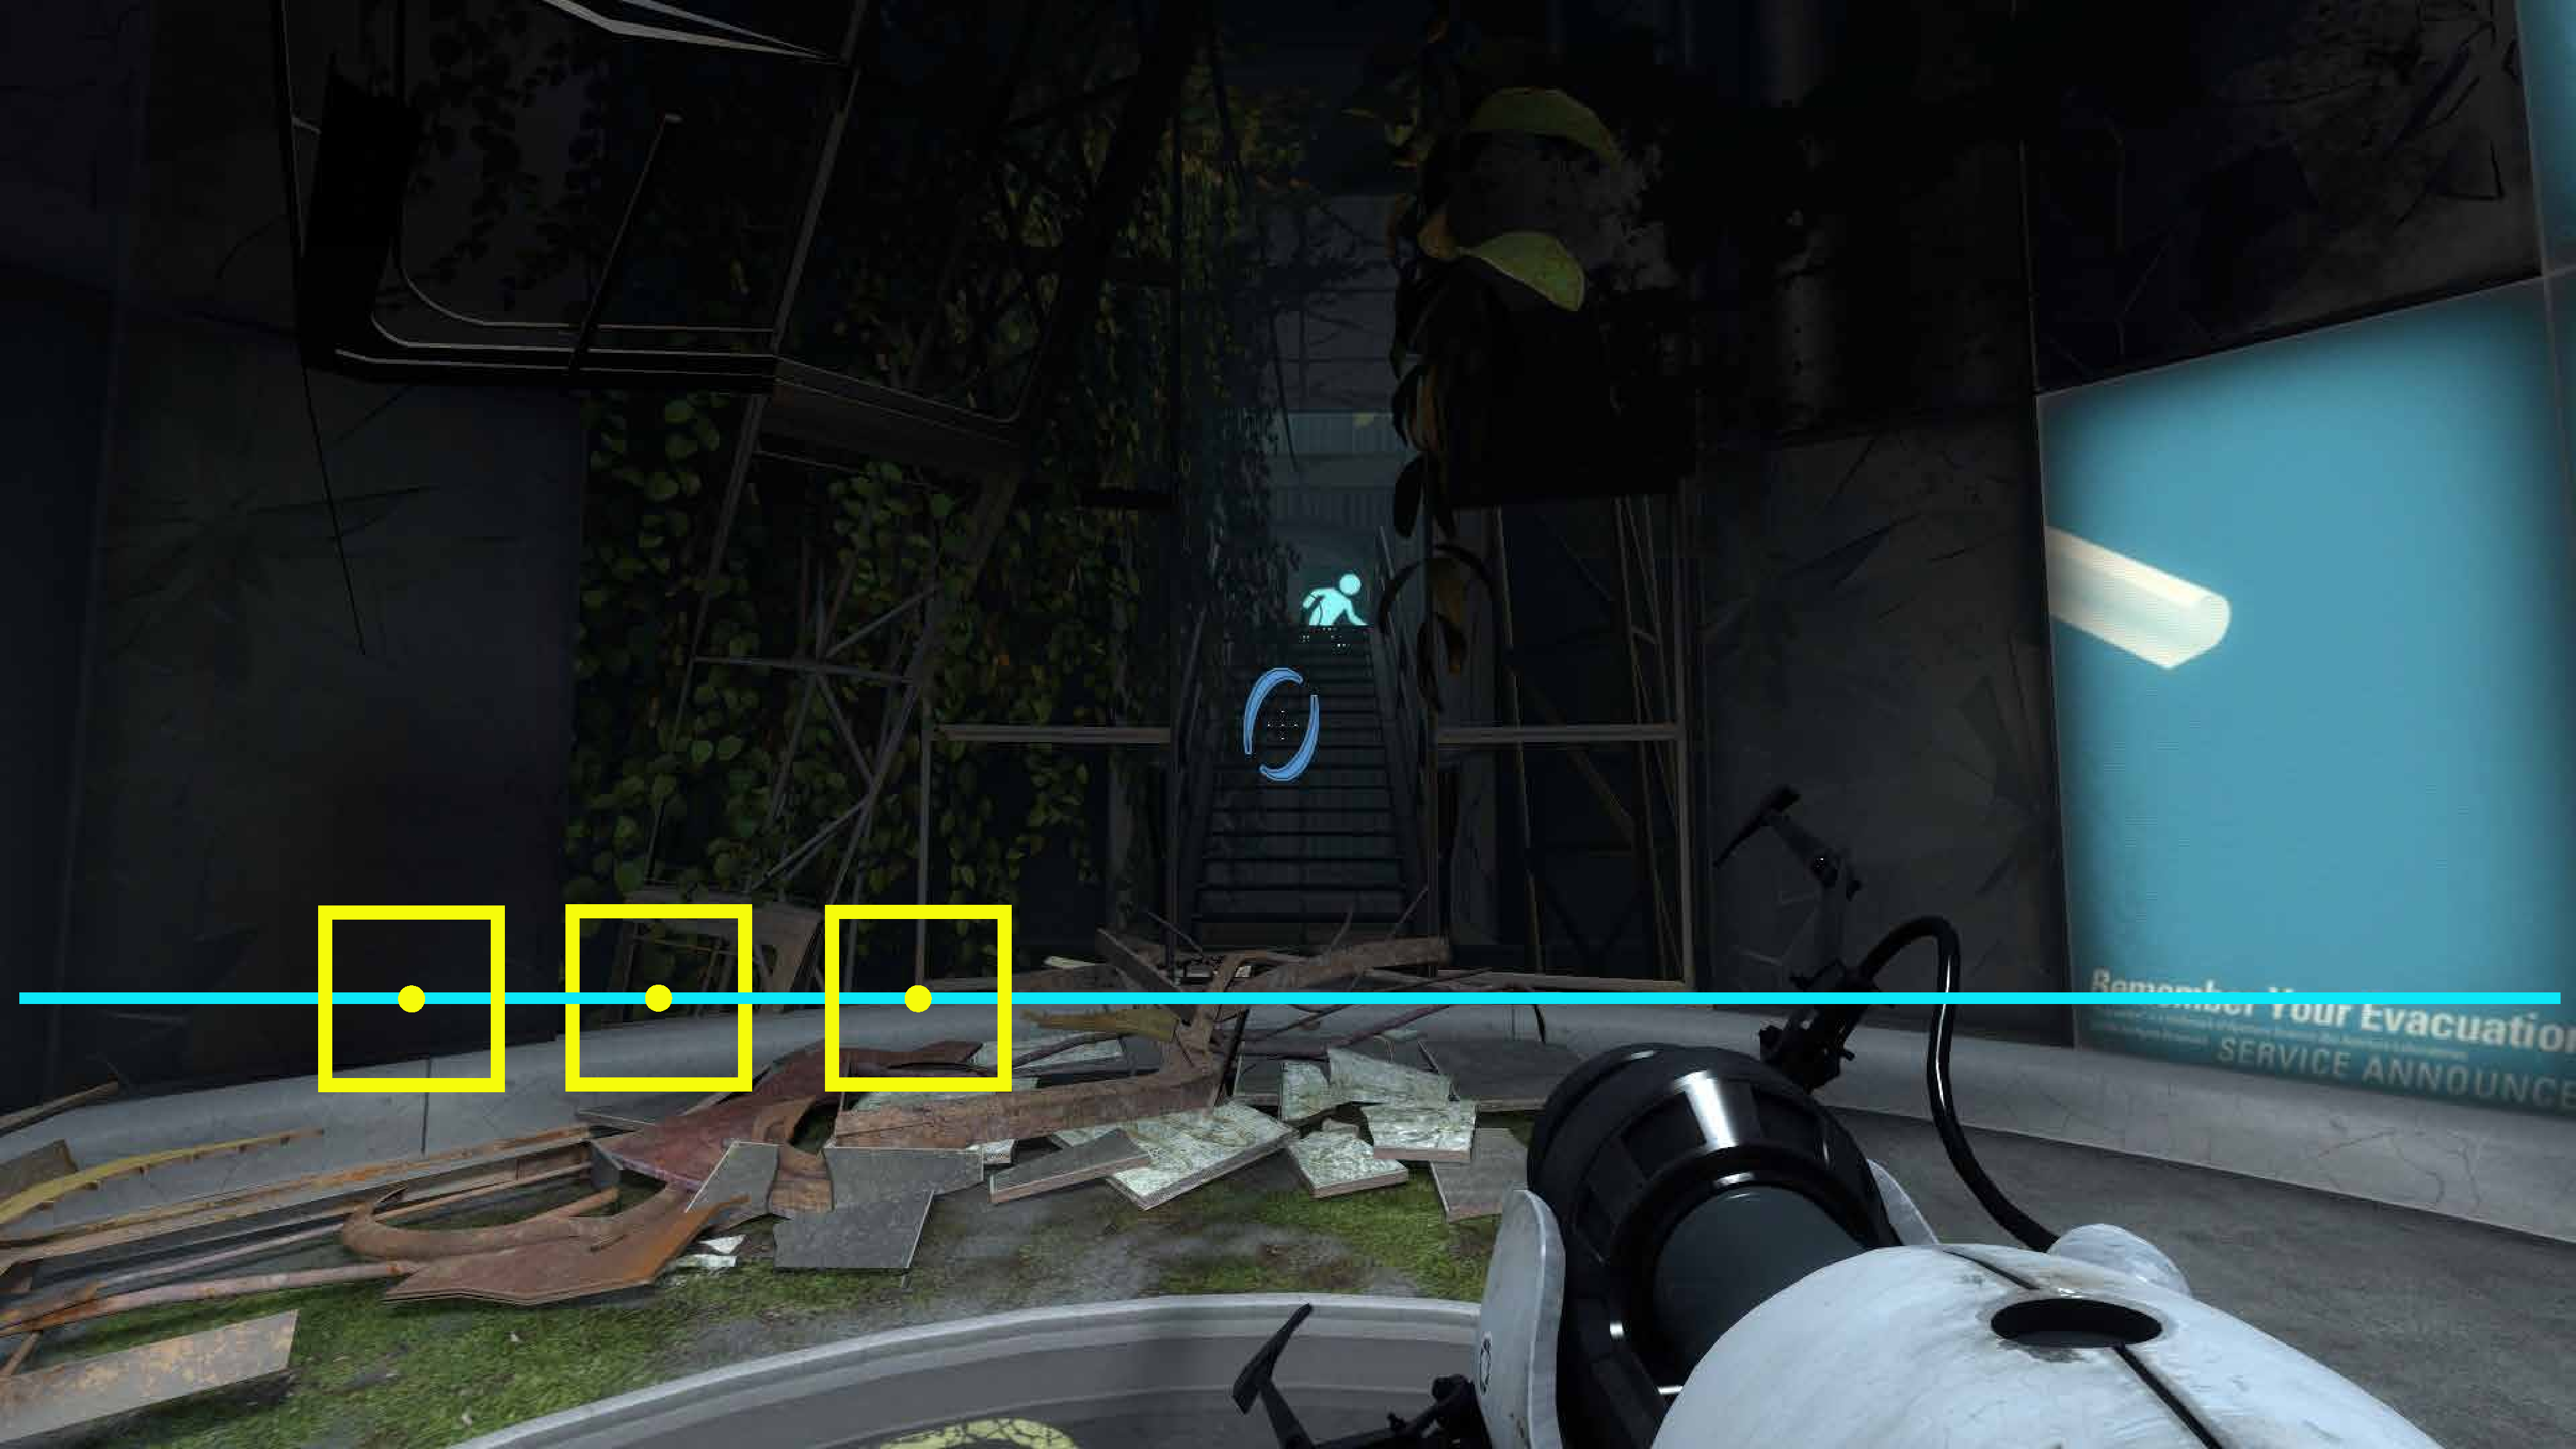
\includegraphics[width=1\linewidth]{figures/part2/search_region1b}
		\caption{Right view}
		\label{fig:search_region1b}
	\end{subfigure}
	\caption{Scanlines and more reasonable search region}
	\label{fig:search_region1}
\end{figure}

Source code of variable window overlap and variable search region geometry are in Appendix \ref{code:2.4}.

\textbf{c). Multi-Pass Cross Correlation}

This process involves doing a course-to-fine multi-stage correlation. Consider the 2-pass cross correlation shown in Figure \ref{fig:multi_pass} as an example. In simple terms, the first pass is a broad guess at where the object has moved to and the second pass takes the information from this guess and provides finer detail.

For the first pass, the search region in the right image is centered at the same location as the template in the left image. This returns a pair (dpx, dpy) which is used to estimate center for the second pass.

In the second pass, the template was split to 4 smaller templates and search region in the right image is centered at the location of the template plus (dpx, dpy) and it returns 4 new centers for next pass.

\begin{figure}[h!]
	\centering
	\begin{subfigure}[t]{0.48\linewidth}
		\centering
		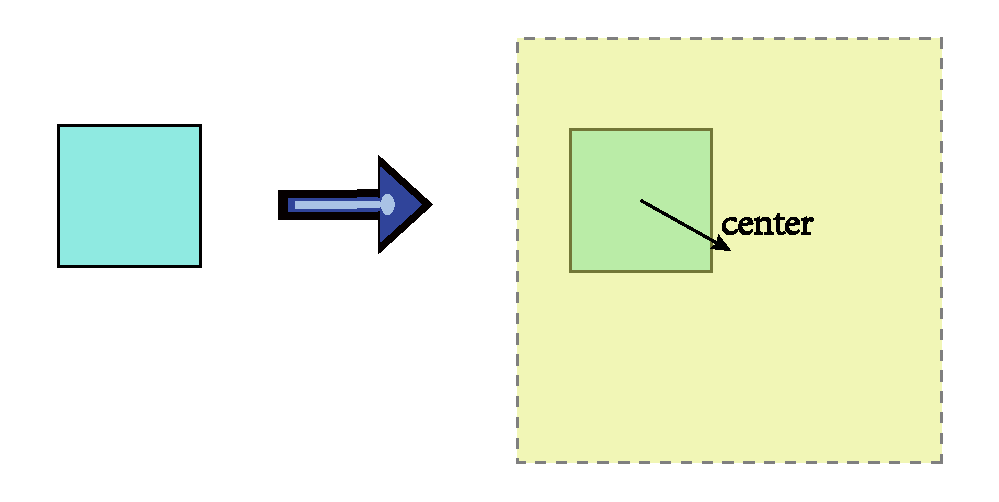
\includegraphics[width=1\linewidth]{figures/part2/multi_pass1}
		\caption{1st pass, wsize = 64}
	\end{subfigure}
	\begin{subfigure}[t]{0.48\linewidth}
		\centering
		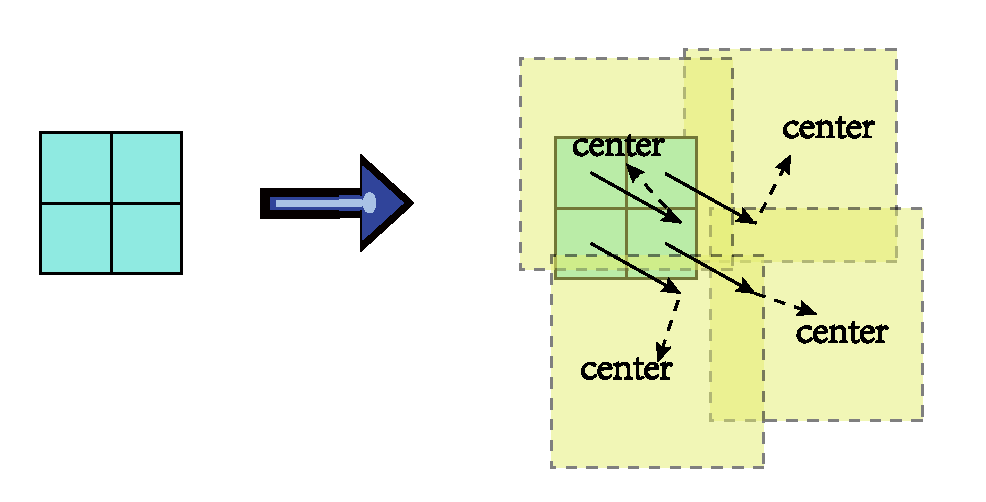
\includegraphics[width=1\linewidth]{figures/part2/multi_pass2}
		\caption{2nd pass, wsize = 32}
	\end{subfigure}
	\caption{Multi-pass cross correlation. (``center'' in the image refer to the new search region's center, yellow square represents new search regions.)}
	\label{fig:multi_pass}
\end{figure}

However, Multi-pass has its flaw. Once the first pass computes a bad shift distance, the second pass will be influenced by this and tend to get a worse shift distance.

Source code of multi-pass cross correlation optimization is in Appendix \ref{code:2.5}.

\section{Test Scan on Computer Generated Calibrated Images}

In this section, we create 3D reconstruction of some test image pairs use fit functions and calibration model. Figure \ref{fig:test_scan} shows the 3D reconstruction on one test image pairs. Figure \ref{fig:test1} and Figure \ref{fig:test2} are computer generated calibrated images from two views. Figure \ref{fig:test3} is the image comparison result, Figure \ref{fig:test4} is reconstructed objects in 3D space and Figure \ref{fig:test5} is a clearer visualization of it. More results on other test sets are in Appendix \ref{fig:all_test_scan}.

\begin{figure}[h!]
	\centering
	\begin{subfigure}[t]{0.3\linewidth}
		\centering
		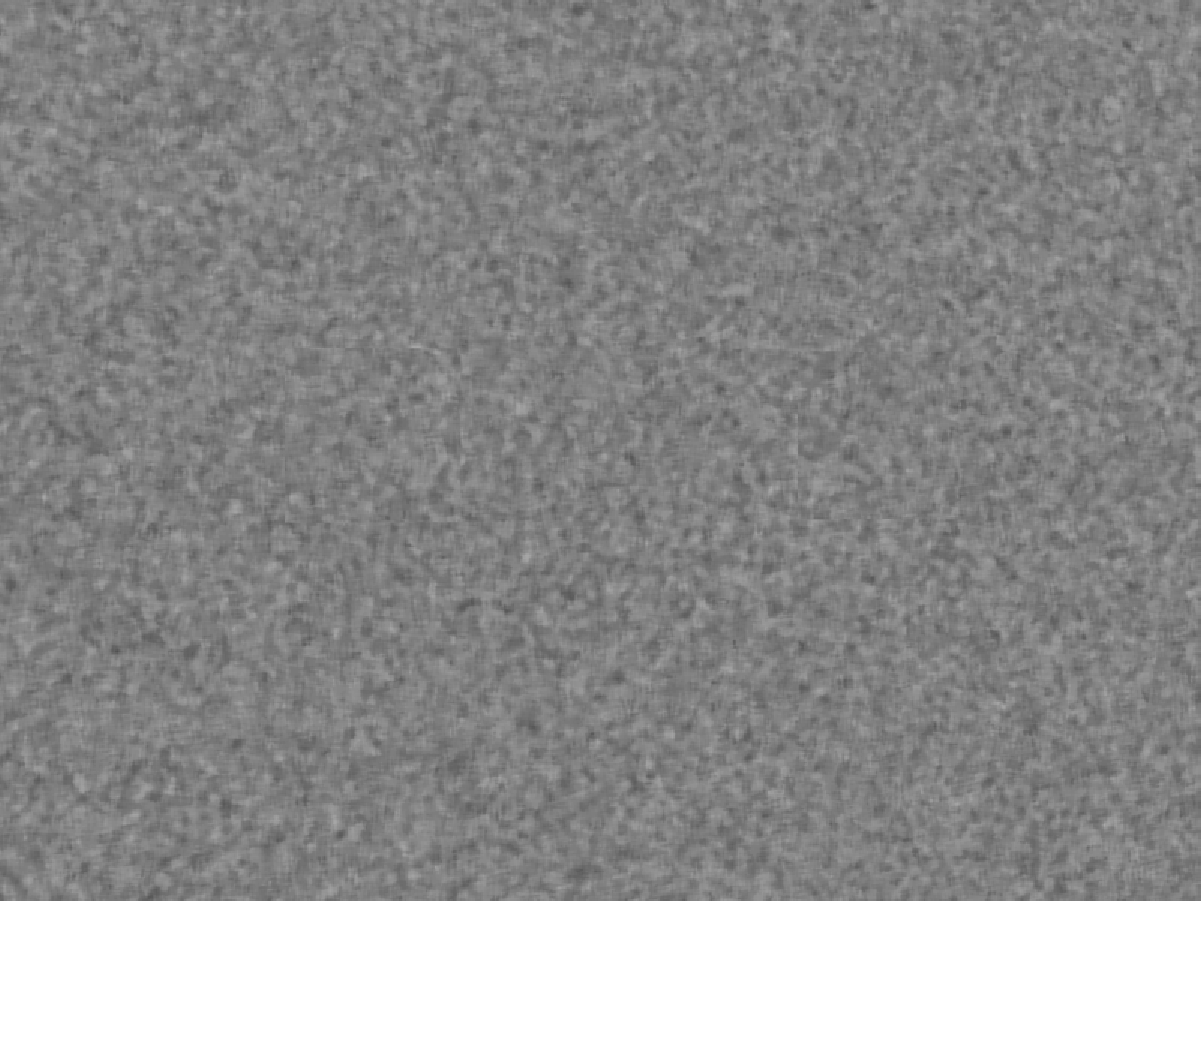
\includegraphics[width=0.8\linewidth]{figures/part2/test_left_2}
		\caption{left}
		\label{fig:test1}
	\end{subfigure}
	\begin{subfigure}[t]{0.3\linewidth}
		\centering
		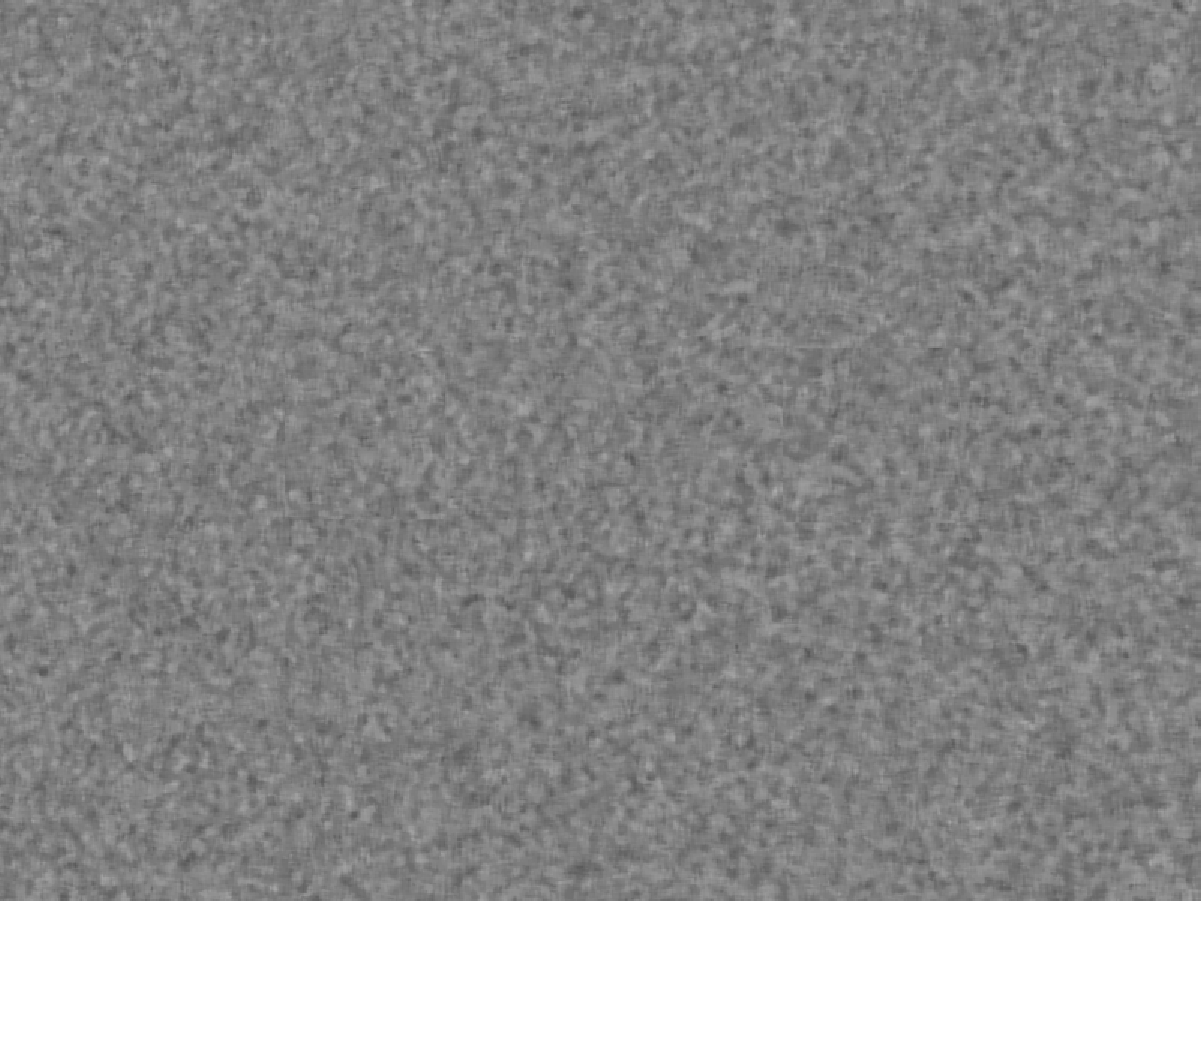
\includegraphics[width=0.8\linewidth]{figures/part2/test_right_2}
		\caption{right}
		\label{fig:test2}
	\end{subfigure}
	\begin{subfigure}[t]{0.35\linewidth}
		\centering
		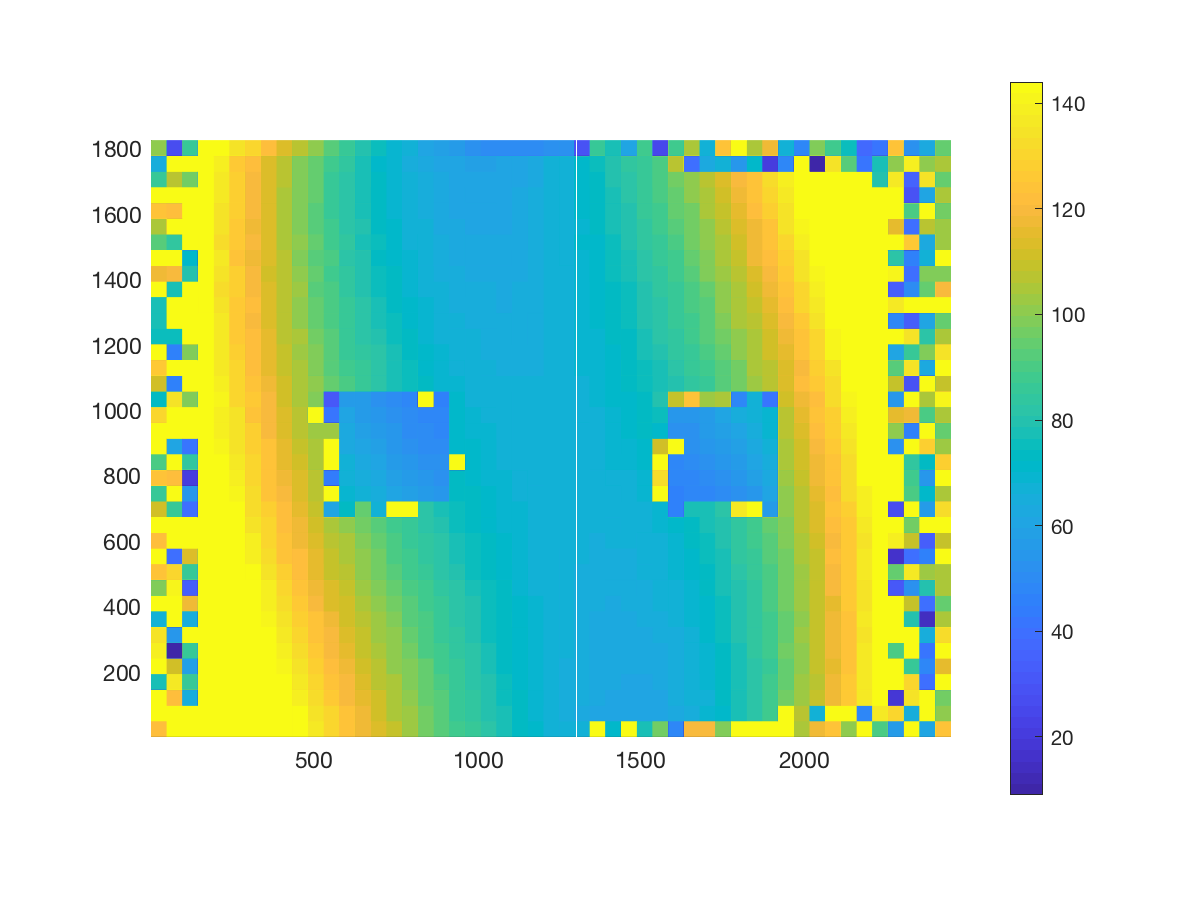
\includegraphics[width=1\linewidth]{figures/part2/test2_cmp}
		\caption{compare result}
		\label{fig:test3}
	\end{subfigure}
	\begin{subfigure}[t]{0.45\linewidth}
		\centering
		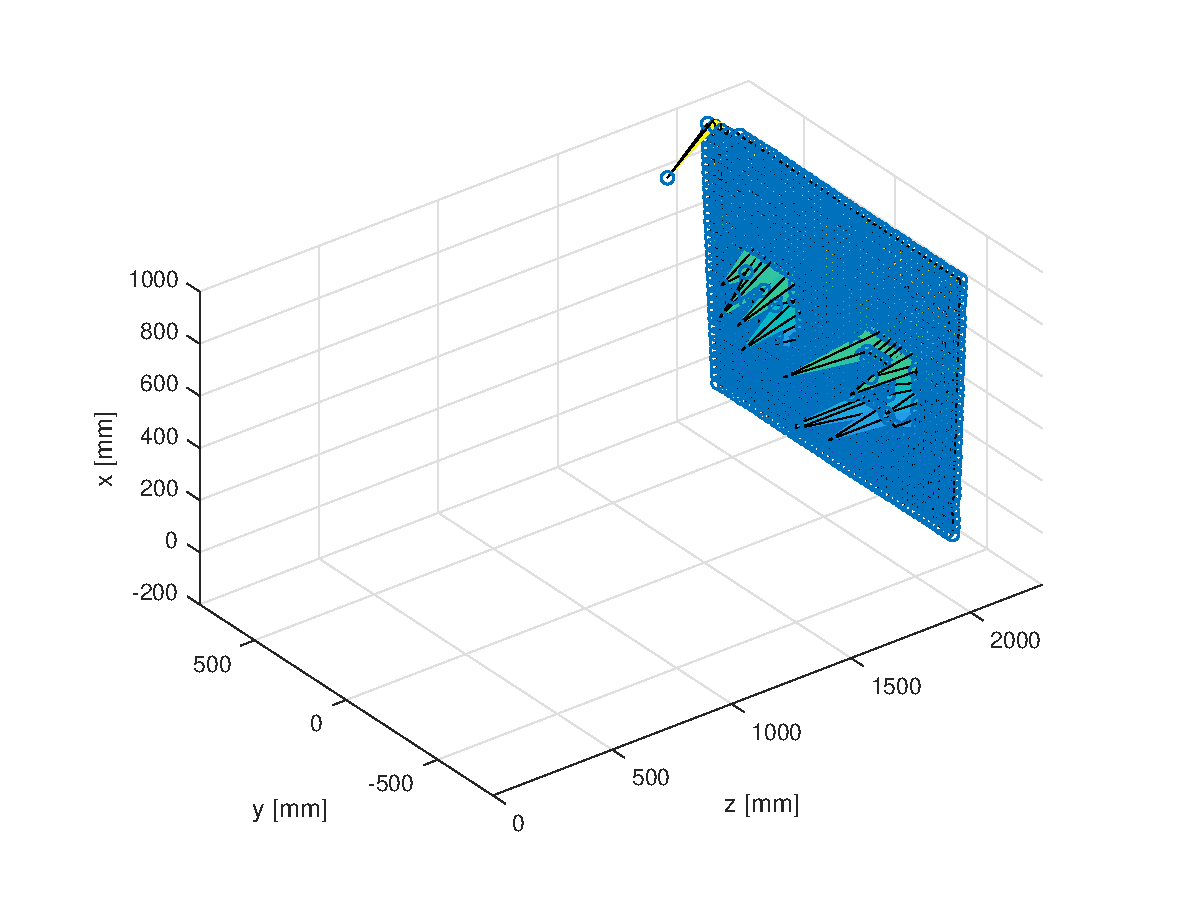
\includegraphics[width=1\linewidth]{figures/part2/test2_scan}
		\caption{3D reconstruction}
		\label{fig:test4}
	\end{subfigure}
	\begin{subfigure}[t]{0.45\linewidth}
		\centering
		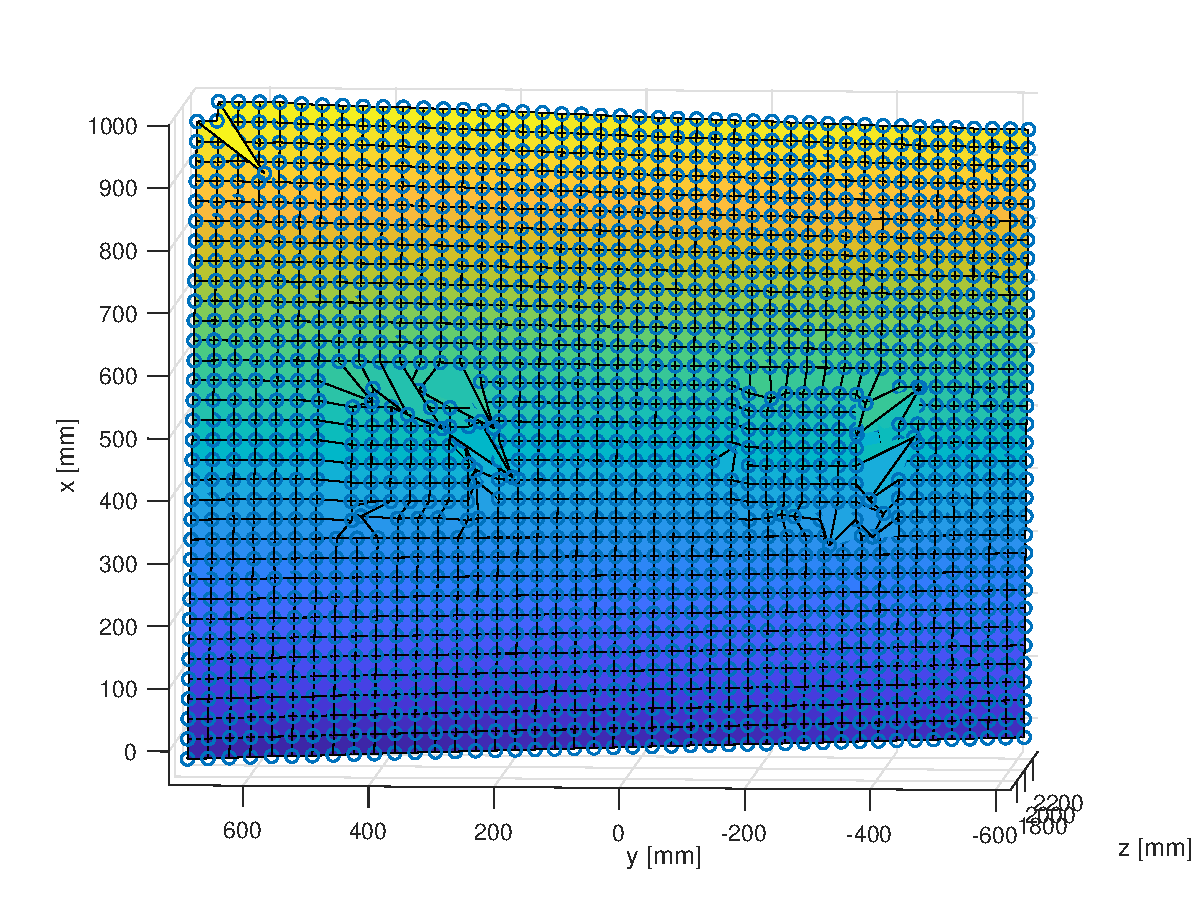
\includegraphics[width=1\linewidth]{figures/part2/test2_scan1}
		\caption{3D reconstruction}
		\label{fig:test5}
	\end{subfigure}
	\caption{Test scan on computer generated calibrated images}
	\label{fig:test_scan}
 
\end{figure}


From the above images we find that the image comparison does not work well at the edge of images of the second and third test pairs. So we remove these vectors to get a more reasonable 3D reconstruction although there are still spurious exist. 

Source code for 3D reconstruction is in Appendix \ref{code:2.6} and \ref{code:2.7}. There are many limitations of the program. First, we implement two versions code for test 1, and others. For test1, we use dot detection algorithm which return all dots' position in two images. For test 2 and 3, we use image comparison algorithm but it dose not work well at the edge of the images. 


\section{Optimized Test Scan}

In this section, some optimization optionals of reconstruction 3D scenery are investigated, Actually, the plots shown in Figure \ref{fig:test_scan} are optimized reconstruction results. Figure \ref{fig:scan_op} shows the progress of search region's optimizations. Figure \ref{fig:scan_op_a} is the result of 1,5x flat search region and Figure \ref{fig:scan_op_b} is the result of 1.5x square region. We can find results on square search region performs better than results on flat search region if search region is small. Figure \ref{fig:scan_op_c} is the result of 3x square search region, we find it is better than the result of 1.5x square search region. It may because the larger search region could return a more precise results, of course it costs more time. 

\begin{figure}[h!]
	\centering
	\begin{subfigure}[t]{0.3\linewidth}
		\centering
		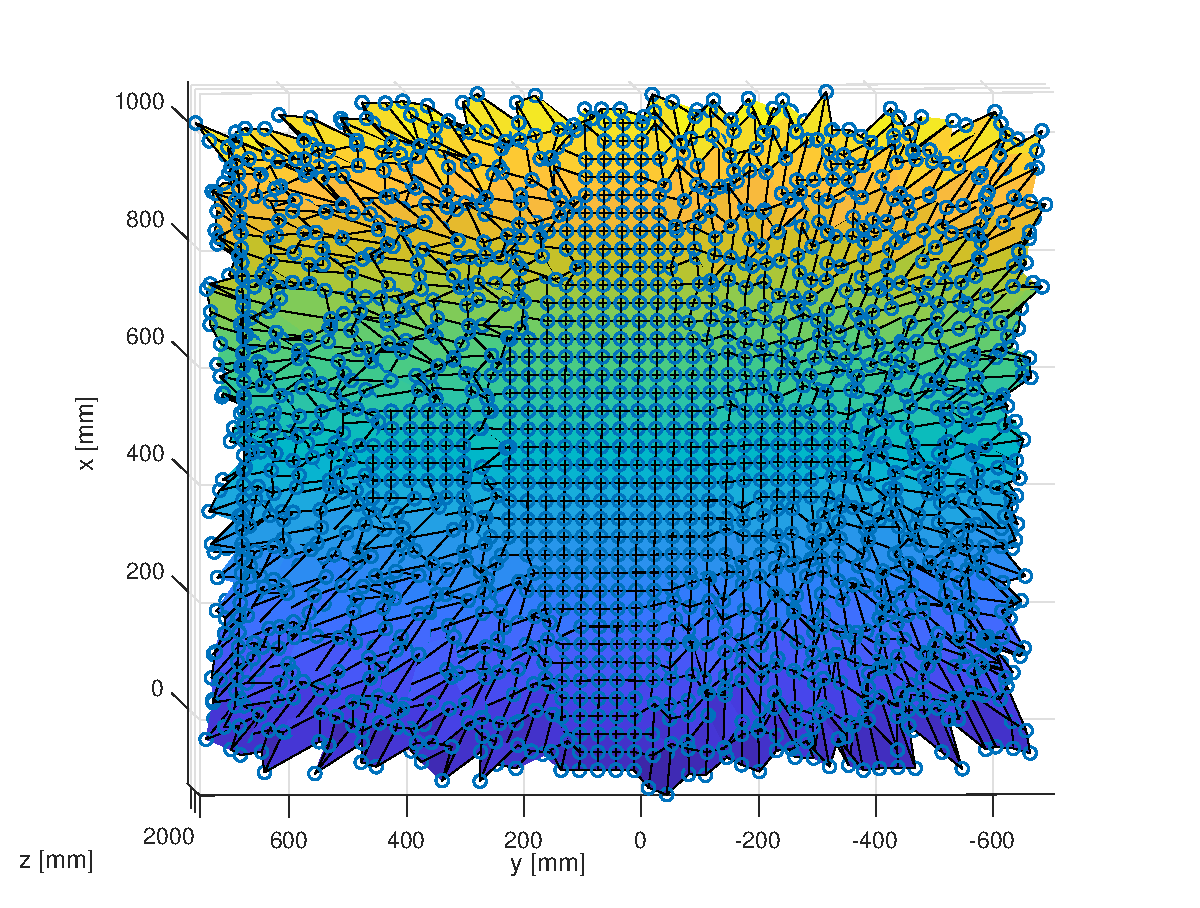
\includegraphics[width=1\linewidth]{figures/part2/scan2f}
		\caption{1.5x flat search region}
		\label{fig:scan_op_a}
	\end{subfigure}
	\begin{subfigure}[t]{0.3\linewidth}
		\centering
		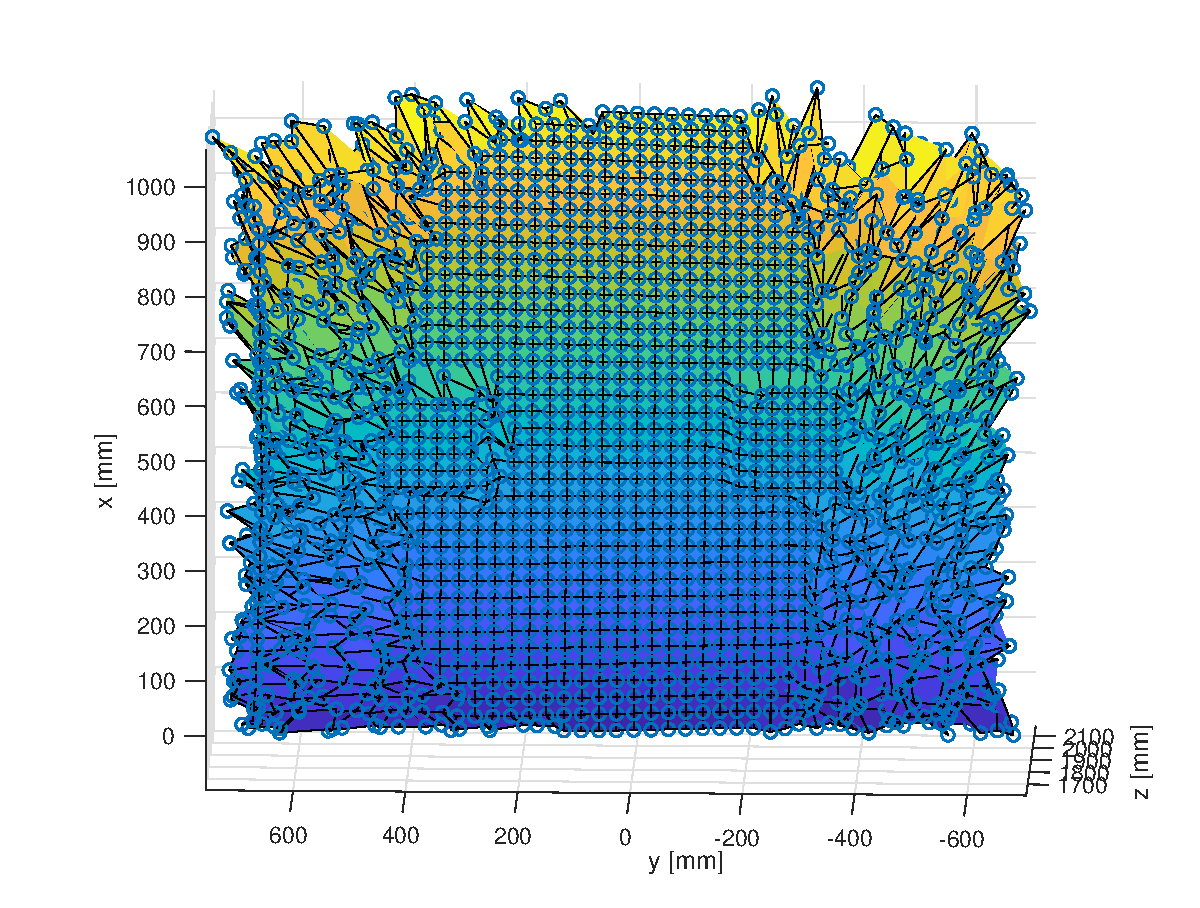
\includegraphics[width=1\linewidth]{figures/part2/scan2}
		\caption{1.5x square search region}
		\label{fig:scan_op_b}
	\end{subfigure}
	\begin{subfigure}[t]{0.3\linewidth}
		\centering
		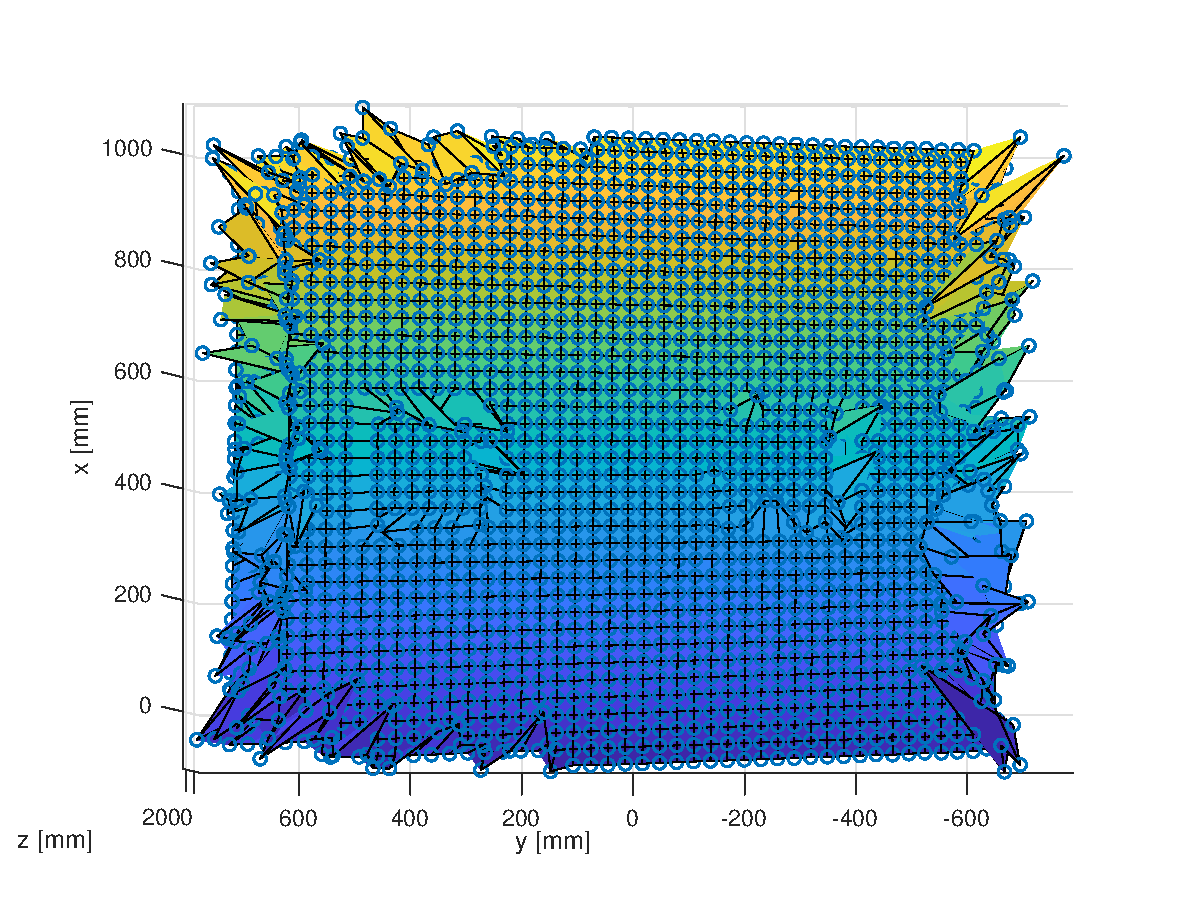
\includegraphics[width=1\linewidth]{figures/part2/scan3}
		\caption{3x square search region}
		\label{fig:scan_op_c}
	\end{subfigure}
	\caption{Optimization of scan test}
	\label{fig:scan_op}
\end{figure}

In addition to image comparison optimization, calibration model could be optimized through a more accurate dot detection algorithm, that is, sub-pixel level dot detection. Sub-pixel techniques have been was presented by Hueckel M F\cite{Hueckel1973A} and widely used in many image processing \cite{Avrahami1991Sub}\cite{Haskett2001Ares}\cite{Huertas2009Detection}. 

In this task, cross correlation $X$ between calibration plate and gaussian template will be computed first. Different with dot detection in task 1, one peak detected in $X$ (position with maximum value) would be treat as a part of one locking peak rather a detected dot. The whole part of locking peak is a range which center is the detected peak, as shown in Figure \ref{fig:sub_pixel}. The central yellow square is the detected peak whose coordinate is $(4,4)$ in this locked range (whole part). We compute the center of gravity weighted by the value of each pixel. Figure \ref{fig:weight} demonstrate the strategy in one dimension.  In Figure \ref{fig:weight}(1), the center of gravity is coincide with the geometric center because the vector value is symmetrical. While in Figure \ref{fig:weight}(2), the center of weight located on the right of the geometric center because the right part have higher value than left part, which gives them more weight. The method can easily extend to two dimensions and be used to find sub-pixel position of the maximum value.

\begin{figure}[h!]
	\centering
	\begin{subfigure}[t]{0.48\linewidth}
		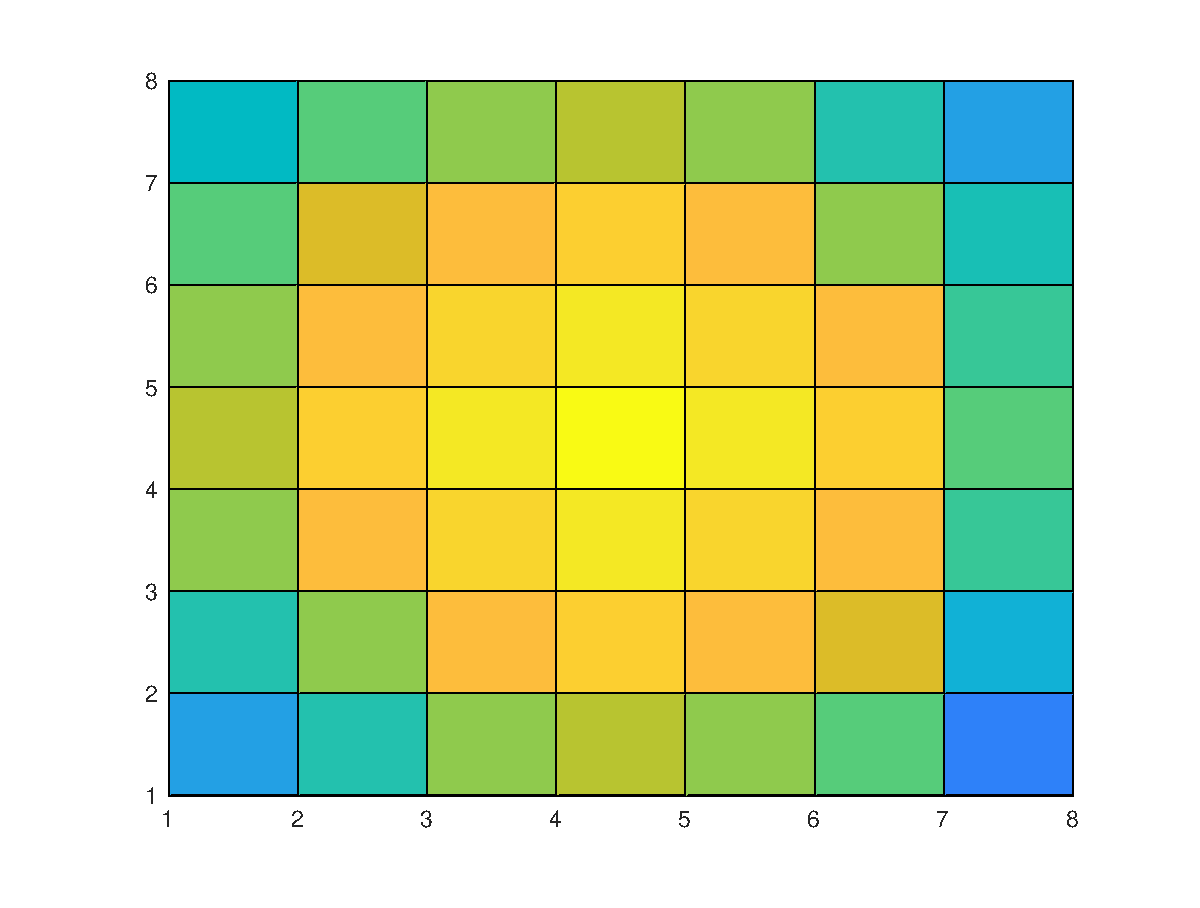
\includegraphics[width=1\linewidth]{figures/part2/sub_pixel}
		\caption{Surf plot of locked peak.}
		\label{fig:sub_pixel}
	\end{subfigure}
	\begin{subfigure}[t]{0.48\linewidth}
		\centering
		
\includegraphics[width=1\linewidth]{figures/part2/weight1}
		\caption{Demonstration of center of gravity weighted by value, red dots is the center.}
		\label{fig:weight}
	\end{subfigure}
	\caption{Sub-pixel dot detection method}
\end{figure}

Source code of sub-pixel level dot detection is in Appendix \ref{code:2.8}. 

\section{Better Calibration model}

In this chapter, we build a calibration model and combine it with image comparison and finally reconstruct a 3D objects of images. There are some thinking of myself. 

The built calibration model is based on the function fitting of several calibration plates. Although these plates distribute in different place in 3D space. They cover a little space of viewable range. So it works well only if the reconstructed objects in this little area. In this project, maybe $x\in (0,1000)$, $y\in (-500,500)$ and $z\in (1900,2000)$. However, in our daily life, we want the depth information from some pictures took by camera, and the distance of the scenery may vary form 0 to very large number. The model proposed in the project may fail to this general task. 

In my opinion, there are some solutions. The first one is use 3D calibration objects, actually, this idea is similar with using several 2D calibration plates with various $z$ value. But use several 3D calibration objects may get more accurate calibration because it provides continuous fit sample for functions. Actually, maybe this method does not be mentioned because of the coding difficulty. The second approach is using several cameras. They do not have to be put in the same horizontal level, on the contrary, they can be put in the four corners of a rectangle. Multi cameras give both robustness and precision of the model. Of course there should be better solutions, these two are just some thinking of my.

